\documentclass[12pt,a4paper]{scrartcl}

\usepackage[utf8]{inputenc}
% \usepackage[latin1]{inputenc} %  Alternativ unter Windows
\usepackage[T1]{fontenc}
\usepackage[ngerman]{babel}

\usepackage[pdftex]{graphicx}
\usepackage{latexsym}
\usepackage{amsmath,amssymb,amsthm}

% Links einbinden:
\usepackage[colorlinks=true,urlcolor=blue,citecolor=blue,linkcolor=blue]{hyperref}

% SI-Units einbinden:
\usepackage{siunitx}
\sisetup{locale = DE ,per-mode = symbol}

\usepackage{hyperref}

% Abstand obere Blattkante zur Kopfzeile ist 2.54cm - 15mm
\setlength{\topmargin}{-15mm}


\begin{document}

  % title page and tabel of contents
  \pagestyle{empty}
  \begin{titlepage}

    \par
    \raisebox{-.5\height}{
\includegraphics[scale=0.5]{images/0_kit-logo.jpg}}%
    \hfill
    \raisebox{-.5\height}{
\includegraphics[width=2cm]{images/ifv_logo.png}}%
    \par

    \vspace*{1cm} 

    \begin{center} \large 
    
        Seminararbeit \\
        im \\
        Seminar Verkehrswesen
    
        \vspace*{2cm}

        {\huge Stauindex}
        \vspace*{2.5cm}

        Markus Scherer\\
        Christof Urbaczek\\
        Nils Hennemann
    
        \vspace*{1.0cm}

        \today
        \vspace*{2.5cm}

        Betreuung:\\
        Dr.-Ing. Bastian Chlond\\
        M.Sc. Sascha von Behren \\[1cm]

        Fakultät für Bauingenieurwesen \\
        Institut für Verkehrswesen \\
        Karlsruher Institut für Technologie

    \end{center}
  \end{titlepage}

  \tableofcontents
  \newpage
 
  % report content
  \pagestyle{headings}
  \section{Motivation und Zielsetzung}

Die Untersuchung der Verkehrssituation eines (Siedlungs-)Gebietes stellt eine zentrale Aufgabe der strategischen Verkehrsplanung dar. Mögliche Zielsetzungen können hierbei die reine Quantifizierung der aktuellen Verkehrsverteilung, die Entwicklung einer Verkehrsprognose oder die Bewertung einer verkehrlich bedeutsamen (Bau-)Maßnahme sein. Um eine verlässliche Aussage über die Belastungen auf den Verkehrsnetzen eines Siedlungsraumes zu ermitteln, ist die Entwicklung eines Verkehrsmodells heute gängige Praxis.\\

Bevor eine entsprechend aufwendige und teils langwierige Entwicklung eines Verkehrsmodells in Angriff genommen werden kann, ist eine ausführliche Voruntersuchung notwendig und es bedarf einer umfangreichen Grundlage an Strukturdaten, Verhaltensdaten, Verkehrskennzahlen und vielem mehr. In diesem Stadium der Untersuchung fehlt dem Planer bisher ein wirkungsvolles Tool, welches es ihm ermöglicht, eine Verkehrssituation schnell und automatisiert erfassen zu können.\\

Die vorliegende Seminararbeit setzt sich als Ziel, ein solches Tool zu entwickeln und dessen Möglichkeiten und Grenzen zu untersuchen. Hierzu soll alleine auf Basis öffentlich zugänglicher Online-Kartendienste eine Routine entwickelt werden, welche die Flächennutzung, die aktuelle Verkehrssituation sowie deren zeitliche Veränderung in einem Untersuchungsgebietes automatisiert ermittelt.\\

Im folgenden Kapitel wird zunächst auf die technische Umsetzung und Implementierung des Tools eingegangen. Es werden die Vor- und Nachteile verschiedener Kartendienste genannt und deren Eignung als Grundlage für die vorliegende Untersuchung ausgelotet. Des Weiteren wird beschrieben, wie die gesammelten Daten aus den Kartenelementen gewonnen, analysiert und schließlich visualisiert werden können. Das entwickelte Verfahren wird im daran anschließenden Kapitel auf ein Beispiel angewendet, um die wählbaren Parameter und deren Einfluss auf das Ergebnis im Rahmen einer Sensitivitätsanalyse abzuschätzen. Darauf aufbauend wird ein standardisiertes Vorgehen zur Schaffung einer einheitlichen Datenbasis abgeleitet. Diese findet Anwendung im darauffolgenden Kapitel, in welchem das Tool genutzt wird, um die Verkehrs- und insbesondere die Stausituation verschiedener Siedlungsgebiete zu analysieren und daraus für diese einen vergleichbaren Stauindex zu generieren.

  \newpage
  \section{Technische Umsetzung}

Ziel dieses Seminars war die Auslotung von Möglichkeiten die Daten öffentlich zugänglicher Quellen zu nutzen, um für fest definierte Untersuchungsgebiete erste Bewertungen der Verkehrssituation vorzunehmen. Diese Informationen können dazu dienen die Verkehrssituation auf einzelnen Streckenabschnitten zu untersuchen oder eine Bewertungsgrundlage zur Beurteilung bestehender Maßnahmen auf städtplanerischer Ebene zu schaffen. Vor allem in der Voranalyse kann dies Verkehrsplanern helfen einen ersten Überblick über die Verkehrssituation eines neuen Untersuchungsgebiet zu erhalten und damit erste Rückschlüsse auf Zusammenhänge und Problemfelder zuzulassen, die im Folgenden genauere untersucht werden können.\\

Das entwickelte Tool konzentriert sich auf die Ermittlung und Bewertung von öffentlich zugänglichen Verkehrsdaten und ermöglicht durch Momentaufnahmen und längeren Untersuchungszeiträumen eine erste Beurteilung der zeitlichen Entwicklung der Verkehrssituation innerhalb des definierten Untersuchungsgebiets. Angereichert werden diese Daten mit Flächeninformationen, die erste Rückschlüsse auf den Bebauungsgrad sowie die bestehende Infrastruktur geben und die zusätzlich zur Eingrenzung des Untersuchungsgebiets genutzt werden können.\\

Die Anforderungen jeder Untersuchung sind sehr individuell, weswegen bei der Entwicklung darauf geachtet wurde, dass stets sowohl bei der Datenerfassung wie auch der Datenanalyse die Untersuchungsparameter beim Programmaufruf eingestellt werden können. Somit ermöglicht das Tool sowohl makroskopische Betrachtungen wie beispielsweise die Bewertung der Verkehrssituation einer Stadt ebenso wie die Untersuchung ausgewählter Streckenabschnitte oder einzelner Straßen.

\subsection{Auswahl der verwendeten Kartendienste}
\label{sec:kartendienste}

Zur Erfüllung der individuellen Anforderungen musste auch der verwendete Kartendienst entsprechende Kriterien erfüllen, damit die Daten an die Untersuchung angepasst werden konnten.  Wichtigstes Kriterium war dabei der automatisierte Download des Kartenmaterials. Nur über einen automatisierten Prozess können zeitliche Verläufe -- vor allem über einen längeren Zeitraum -- zuverlässig aufgezeichnet und untersucht werden, die Generierung von Screenshot oder ähnliche Vorgehensweisen hätten diese Arbeit behindert. Aufgrund der Datenmenge und aufgrund rechtlicher Gründe stellt zudem kein Kartenanbieter sein vollständiges Kartenmaterial zur Verfügung, was dazu führt, dass Kartenausschnitte je nach Größe aus einzelnen Segmenten zusammengefügt werden müssen. Das genaue Vorgehen wird im Kapitel \ref{sec:kachelsystem} genauer beschrieben, es erfordert allerdings speziell bei der Verkehrsanalyse den synchronen Download mehrerer Aufnahmen und könnte manuell kaum geleistet werden. Neben der Automatisierung mussten zudem die Anforderungen der einzelnen Programmbausteine beachtet werden. Während bei der Flächenanalyse vor allem geometrisches Kartenmaterial benötigt wird, das mit der jeweiligen Flächennutzung verknüpft ist, ist bei der Verkehrsanalyse vor allem der Zugang zu aktuellen Schnappschüssen der Verkehrssituation wichtig, der mit dem bestehnden Kartenmaterial verknüpft werden kann.\\

Bei der Recherche geeigneter Kartendienste wurden die Anbieter \href{https://www.google.de/maps/}{GoogleMaps}, \href{https://www.bing.com/maps/}{BingMaps} und \href{http://www.openstreetmap.org/}{OpenStreetMap} untersucht. Alle drei Dienste stellen statische Schnittstellen bereit und ermöglichen damit den Download einzelner Kartensegmente mit unterschiedlichen Parametern. Zudem ist das Kartenmaterial aller drei Dienste -- innerhalb der jeweiligen Nutzungsbedingungen -- frei zugänglich und können zum Zwecke des Seminars genutzt werden.\\

OpenStreetMap bietet sich als OpenSource-Map für wissenschaftliche Untersuchungen an, da das sehr genaue Kartenmaterial frei zugänglich und uneingeschränkt kostenfrei verfügbar ist. Die Karten entstehen dabei durch die Arbeit tausender freiwilliger Helfer, die den Genauigkeitsgrad der Karten stetig verbessern. Im Gegensatz zu kommerziellen Karten kann es zwar in abgelegenen Orten zu Lücken im Kartenmaterial kommen, die Anforderungen des Seminars beschränken sich allerdings auf die Analyse von Stadtgebieten und Infrastruktur, die Genauigkeiten in diesen Gebieten kann vorausgesetzt werden. Auch wenn das Kartenmaterial umfangreich ist, bietet das System leider keine aktuellen Verkehrsinformationen an. Unabhängige Projekte wie \href{http://opentraffic.io/}{OpenTraffic} versuchen zwar diese Zusatzinformationen ebenfalls als OpenSource-Material zur Verfügung zu stellen, jedoch sind hier noch keinerlei Daten abrufbar (Stand März 2017), was die Daten auf die eigentlichen Kartendaten reduziert. Der Dienst würde sich daher sehr gut für die Flächenanalyse anbieten, der Fokus dieses Seminars lag allerdings in der Ermittlung und Analyse von  Verkehrsinformationen. Die Flächenanalyse dient primär der Voranalyse und der Einschätzung des Untersuchungsgebiets und wird daher vor allem für die Eingrenzung des Untersuchungsgebiets eingesetzt. Auch wenn über die bereitgestellten Schnittstellen Daten sehr feingranular ausgelesen werden können, wäre die Bestimmung einfacher Kennzahlen mit umfangreicher Einarbeitung und zusätzlichen Berechnungen zur Extraktion der Polygoninformationen verbunden gewesen wäre.\\

Im Gegensatz zu OpenStreetMap bietet GoogleMaps eine sehr einfach justierbare und vor allem individuell anpassbare statische Schnittstelle \cite{googlestaticmap}, mit der das vorliegende Kartenmaterial per HTTP-Abruf in Bildform heruntergeladen werden kann. Mit Hilfe der URL-Parameter kann das Kartenmaterial an die Analyseanforderungen angepasst werden, dies reicht vom Aus- oder Einblenden bestimmter Inhalte bis hin zur individuellen Einfärbung ausgewählter Kartenflächen. Das resultierende Bildmaterial bietet einen schnellen wiederverwendbaren Ansatz das Untersuchungsgebiet einzuschätzen und eignet sich daher sehr gut für die Flächenanalyse, das genaue Vorgehen wird im Kapitel \ref{sec:area-analysis} detailierter beschrieben. Während GoogleMaps bei der Onlinenutzung dem Benutzer viele Einstellungs- und Interaktionsmöglichkeiten bietet, beschränkt sich der kostenlose Offline-Service im wesentlichen auf das bereitsgestellte Kartenmaterial. Zusätzliche Informationen in Form zusätzlicher Ebenen wie z.B. Verkehrsinformationen oder öffentliche Verkehrsnetze werden über die statische Schnittstelle seit einiger Zeit nicht mehr ausgeliefert und stehen ausschließlich dem dynamischen Kartensservice zur Verfügung. Wie bereits beschrieben wird allerdings der statische Download benötigt, um einen dauerhaften Service zu gewährleisten, demnach bietet der GoogleMaps-Dienst zwar sehr gut analysierbares Kartenmaterial, aber ebenso wie OpenStreetMap keine verwertbaren Verkehrsinformationen.\\

Microsofts Kartendienst BingMaps nutzt das Kartenmaterial von \href{https://here.com/}{Here} und bietet darüber viele Möglichkeiten auf Karten- und im Gegensatz zu OpenStreetMap und GoogleMaps auch Verkehrsinformationen zuzugreifen. Ebenso wie Google bietete Bing eine anpassbare statische Schnittstelle \cite{bingstaticmap} über die das Kartenmaterial per HTTP-Abruf in Bildform heruntergeladen werden kann. Im Gegensatz zu den anderen untersuchten Diensten ermöglicht Bing die aktuellen Verkehrsinformationen im generierten Kartenabschnitt darzustellen, was eine dynamische Analyse des heruntergeladenen Materials ermöglicht. Mithilfe von Bildanalyseverfahren, wie im Kapitel \ref{sec:traffic-analysis} genauer beschrieben wird, kann somit die aktuelle Verkehrssituation sowie der Verlauf durch mehrfache Aufnahmen bestimmt und genutzt werden. Leider bietet Bing darüber hinaus nur bedingte Einstellungsmöglichkeiten, weshalb eine Flächenanalyse des vorliegenden Kartenmaterials unnötig erschwert werden würde.\\

Alle untersuchten Dienste bieten Vorteile, die nur kombiniert eine brauchbare Lösung für die Umsetzung des Tools bieten. Während die individuelle Einfärbung von GoogleMaps eine schnelle und reproduzierbare Flächenanalyse gewährleistet, bietet nur Bing Karten mit Verkehrsinformationen, aber keinen direkten Zugang zu den Nutzflächen. Die Kombination der beiden Dienste bietet zwar die notwendigen Daten, bringt allerdings zusätzliche Nachteile in der Nutzung mit sich. Sowohl GoogleMaps als auch Bings kostenlose Dienste unterliegen Nutzungbeschränkungen, die eine automatisierte Analyse behindern. Zum einen wird von beiden Anbietern die maximale Abfragemenge pro tag beschränkt und auf den Tag verteilt (Google 25.000 Abfragen \cite{googleusagelimits}, Bing 30.000 Abfragen \cite{bingusagelimits}), was dazu führt, dass bei Services durchschnittlich nur alle 2-3 Sekunken eine Anfrage durchlassen, der Abruf größere Datenmengen wird dadurch deutlich erschwert. Zudem reduzieren beide Anbieter die verfügbare Bildqualität, was vor allem bei der Analyse größerer Flächen zu Problemen führt. Zu diesem Zweck wurde ein eigenes Kachelsystem entwickelt, was in Kapitel \ref{sec:kachelsystem} näher beschrieben. Mit diesem System war es möglich die Restriktionen der Kartenanbieter zu reduzieren und verwertbare Daten zu extrahieren ohne auf die kostenpflichtigen Dienste zurückgreifen zu müssen.\\

\subsection{Kachelsystem}
\label{sec:kachelsystem}

Die statischen Schnittstelle von Google und von Bing liefern bei Aufruf das vorhandene Bildmaterial auf Grundlage der übergebenen Parameter. Wichtigster Parameter dieser Aufrufe ist der Mittelpunkt, der als Längen- und Breitengradangabe das Zentrum des resultierenden Bildes definiert. Über zusätzliche Parameter kann darüber hinaus die Höhe und die Breite des Bildes bestimmt werden. Die Bildgröße entscheidet maßgeblich darüber wie detailiert und umfangreich das Untersuchungsgebiet ist. Die bereitsgestellten maximalen Auflösungen (Google maximal 640x640px \cite{googleusagelimits}, Bing maximal 2000x1500px \cite{bingstaticmap}) reichen allerdings in den meisten Szenarien nicht aus die untersuchten Flächen in ausreichender Auflösung darzustellen, damit eine weiterführende Analyse möglich ist.\\

Google Maps verwendet wie auch Here für ihre Karten die Mercator-Projektion. Mit Hilfe dieser Projektion werden die Breiten- und Längengrade in Pixelkoordinationen des Kartenausschnitts umgerechnet. Ausgehend von einer Basiskachel bei Zoomstufe 0 (siehe Abbildung \ref{fig:pixelcoordinates}) können damit alle Angaben in einen Gleitkomma-Pixelwert umgerechnet werden, der auf der Welt eindeutig ist. Will man nun die Karteninformationen um einen bestimmten Punkt darstellen, muss die Karte mit Hilfe eines Zoomfaktors vergrößert werden. In diesem Fall würde allerdings auch die Datenmenge exponentiell ansteigen, weswegen die Karten in jeder Zoomstufe in quadratische Kacheln zerlegt werden, die Koordinaten können dann eindeutigen Kachelkoordinaten zugeordnet werden.\\
\begin{figure}
\centering
\begin{tabular}{@{}cc@{}}
    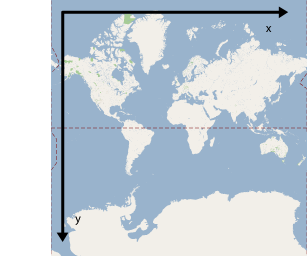
\includegraphics[height=6cm]{images/pixelCoordinates.png} &
    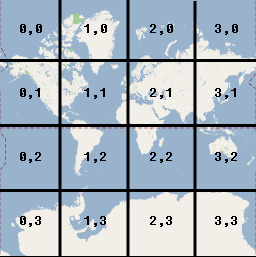
\includegraphics[height=6cm]{images/tileCoordinates.png} \\
\end{tabular}
\caption{Veranschaulichung der Basiskachel bei Zoomstufe 0 (links) und die Einteilung in Kacheln (rechts)}
\label{fig:pixelcoordinates}
\end{figure}

Ausgehend von diesen Überlegungen wurde ein Kachelsystem entworfen, welches von einem definierten Mittelpunkt in einer bestimmten Zoomstufe den Aufbau beliebig großer Kachelmatrizen ermöglicht und damit jedes Untersuchungsgebiet beliebig genau abbilden kann. Durch Hinzufügen weiterer Kachelebenen kann das Untersuchungsgebiet stetig vergrößert und an die Anforderungen angepasst werden. Jede Kachel wird mit der maximalen Auflösung erzeugt und bildet so die größte verfügbare Auflösung für die eingestellte Zoomstufe ab, durch Erhöhung der Zoomstufe kann die Genauigkeit bis zur maximal verfügbaren Zoomstufe (abhängig vom verfügbaren Kartenmaterial) erhöht werden. Dies ermöglicht die Generierung sehr feingranularer Bilder, die als Grundlage weiterer Untersuchungen dienen. Schichten können für ein bereits definiertes Zentrum jederzeit erweitert werden. Die Benamung der Kachelkoordinaten (siehe Abbildung \ref{fig:tilemap}) ausgehend vom Mittelpunkt ermöglicht es dem System bereits ermittelte Kacheln vorzuhalten und den Download neuer Schichten zu beschleunigen. Die statischen Schnittstellen unterstützen solche Kachelabfragen nicht, weswegen das Tool die Berechnungen der Mittelpunkte benachbarter Kacheln übernimmmt und sie selbstständig herunterlädt. Wie Kapitel \ref{sec:verfahrensentwicklung} am Beispiel Karlsruhe erläutert sollte genau auf den gewünschten Detailierungsgrad geachtet werden, denn mit jeder zusätzlichen Kachelschicht müssen $8(n-1)$ zusätzliche Kacheln heruntergeladen und analysiert werden, für eine komplette Kachelmatrix umfasst dies $(2n-1)^2$ Kacheln. Wie bereits in \ref{sec:kartendienste} beschrieben, kann dies zu einem deutlichen Mehraufwand und einige Zeit für den Download in Anspruch nehmen. Vor allem beim Einsatz in der Verkehrsanalyse (siehe \ref{sec:traffic-analysis}) sollte hier darauf geachtet werden, dass die Zeitspanne ausreicht alle Kacheln zu laden bevor ein weiterer Zeitschritt ansteht.
\begin{figure}
\centering
\begin{tabular}{@{}cc@{}}
    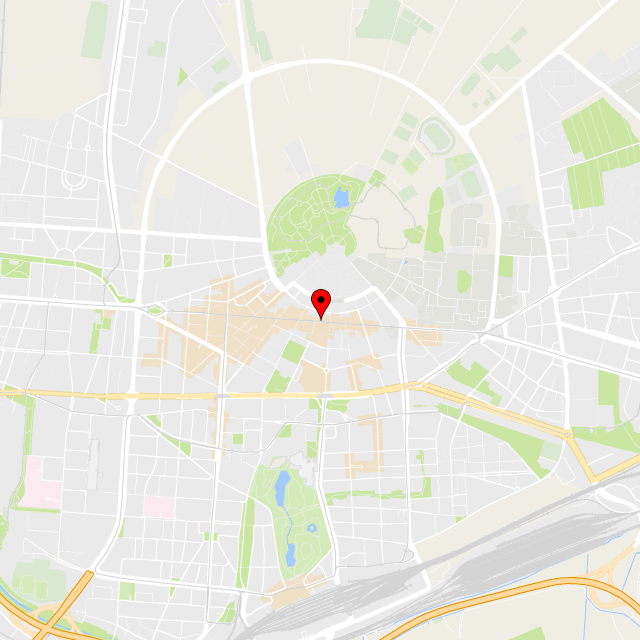
\includegraphics[height=6cm]{images/Karlsruhe_with_center.png} &
    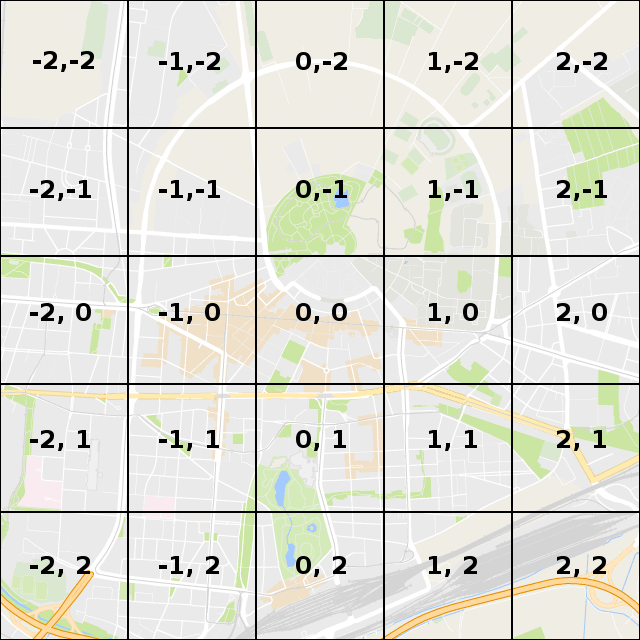
\includegraphics[height=6cm]{images/Karlsruhe_grid.png} \\
\end{tabular}
\caption{Kartenausschnitt der Stadt Karlsruhe mit Zentrumspunkt (links) und eingezeichneter Kachelmatrix (rechts)}
\label{fig:tilemap}
\end{figure}

\subsection{Flächenanalyse}
\label{sec:area-analysis}

Die Flächenanalyse dient der Voranalyse und Einschätzung des untersuchten Gebiets. Durch Anwendung der Analyse auf die einzelnen ermitteltenden Kacheln kann zudem eine Eingrenzung des Suchgebiets erreicht werden. Für die Ermittlung des Kartenmaterials kommt  die statische Schnittstelle von GoogleMaps zum Einsatz, da sich das System aufgrund seiner individuellen Einstellungsmöglichkeiten besonders dazu eignen die gewünschte Flächennutzung auszulesen. Folgende Kennwerte werden bei der Flächennutzung ermittelt:

\begin{itemize}
\item Bebaute Fläche (man-made)
\item Naturfläche (nature)
\item Öffentlicher Verkehr (transit)
\item Straßen (road)
\item Autobahnen und Schnellstraßen (highway)
\end{itemize}

Zum Zwecke einer schnellen und direkten Analyse wurde der Ansatz der Karteneinfärbung genutzt. Dazu werden die umfangreichen Einstellungsmöglichkeiten der GooleMaps API genutzt, um jeden Flächentypen individuell einzufärben. Die API bietet dabei detailierte Einflussmöglichkeiten auf die Flächeneinfärbung, die Darstellung der Beschriftungen sowie auf die Darstellung der Symbole und kann sehr gut den Bedürfnissen für die Bildanalyse vorbereitet werden. Eine darauf folgende Bildanalyse ermöglicht schnell Rückschlüsse auf die Anteile der Flächennutzung einzelner Kacheln wie auch des gesamten Untersuchungsgebiets. Abbildung \ref{fig:ka_area_analysis} zeigt einen Ausschnitt des Karlsruher Bahnhofs samt Umgebung, in der die unterschiedlichen Farbgebungen deutlich werden.\\

Das Tool übernimmt nach Übergabe der wichtigsten Einstellungsparameter die vollständige Analyse. Das System ermittelt in einem ersten Schritt die benötigten Kacheln und lädt sie (falls nicht bereits in einer vorherigen Analyse geschehen) über die Schnittstelle eingefärbt herunter. Die ermittelten Flächenanteile können direkt ausgegeben oder optional in eine CSV-Datei gespeichert werden. Die Generierung der angewendeten Kachelmatrix ermöglicht zudem eine schnelle Übersicht der analysierten Kacheln und ist im Ausschnitt \ref{fig:ka_area_analysis} ebenfalls erkennbar.

\begin{figure}
  \centering
    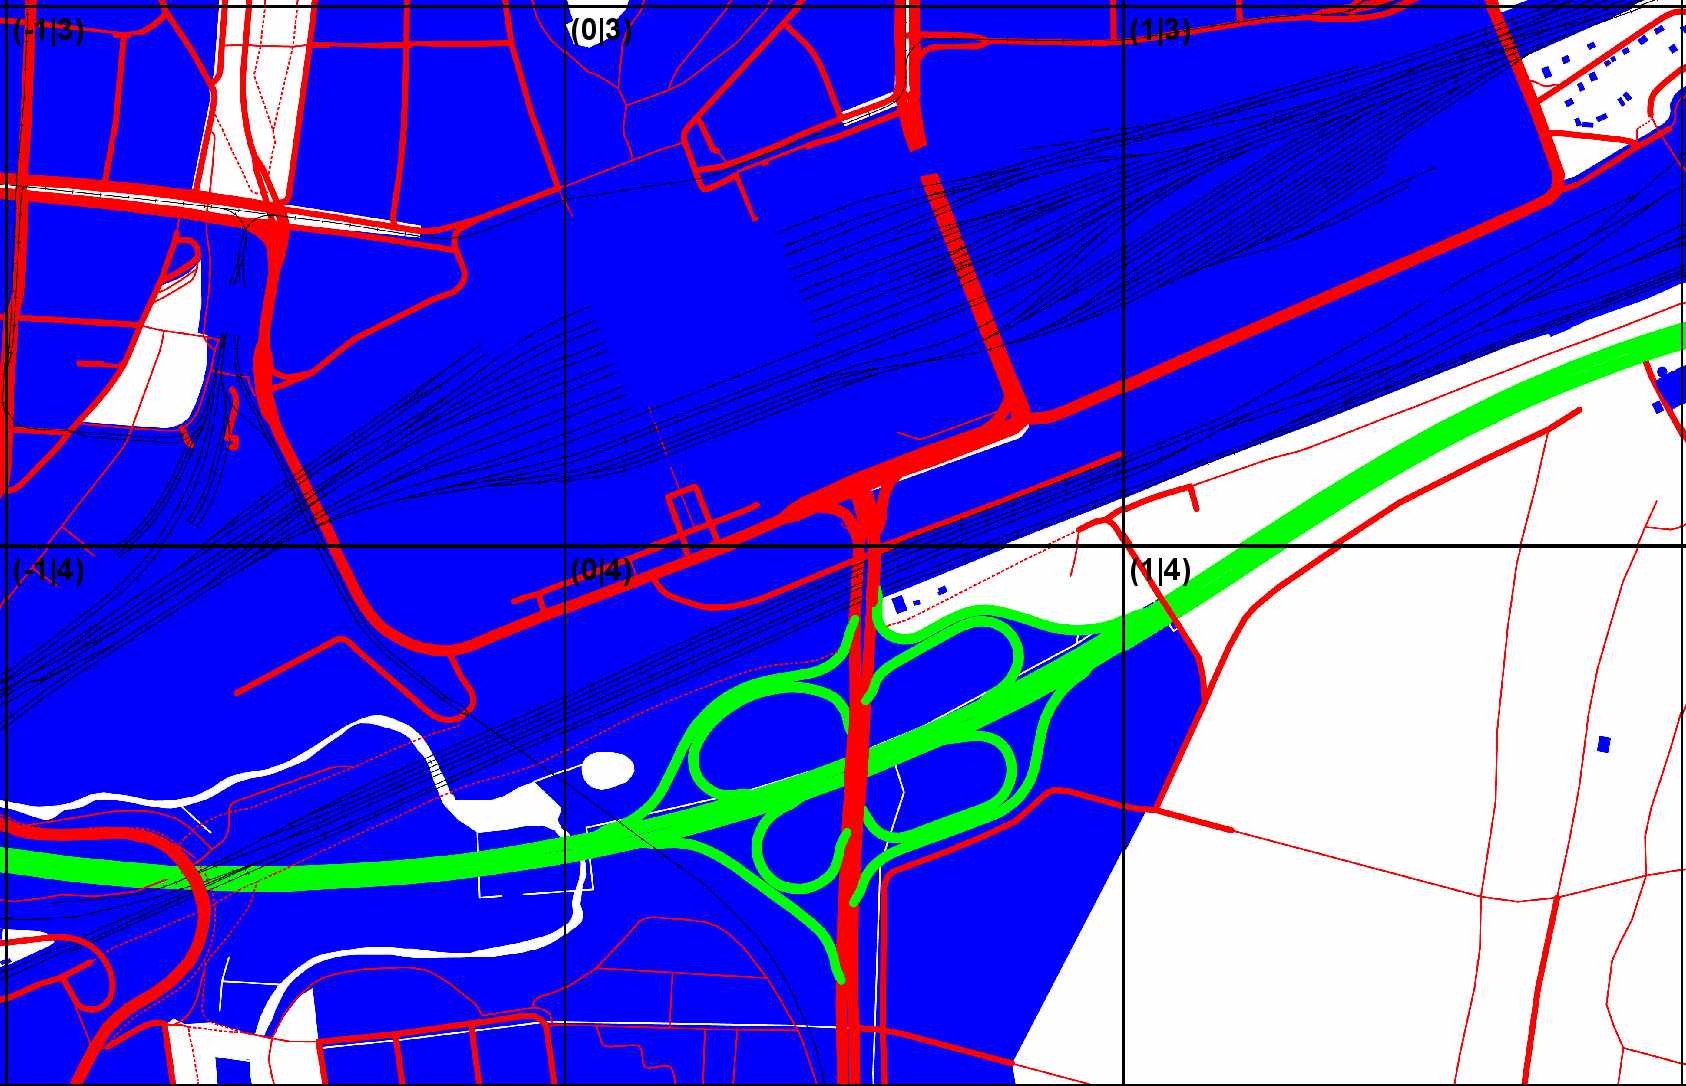
\includegraphics[width=0.9\textwidth]{images/karlsruhe_area_analysis_ausschnitt.png}
    \caption{Ausschnitt der Flächenanalyse der Stadt Karlsruhe auf Zoomstufe 17 und Kachelmenge 5}
    \label{fig:ka_area_analysis}
\end{figure}

\subsection{Verkehrsanalyse}
\label{sec:traffic-analysis}

Die Verkehrsanalyse wird genutzt um Momentaufnahmen oder zeitliche Verläufe der Verkehrssituation innerhalb des Untersuchungsgebiets zu erfassen und zu analysieren. Wie bereits in \ref{sec:kartendienste} dargelegt bietet nur der Kartendienst von Bing eine Schnittstelle, um die Verkehrsinformationen per statischer Schnittstelle auszulesen. Bing bietet ebenso wie Google einige Einstellungsmöglichkeiten beim Kartenabruf aber im Gegensatz zu Google ist keine Einflussnahme auf die direkte Darstellung der Karte möglich. Da das Kartenmaterial nicht so effektiv verarbeitet werden kann wie das von Google muss die Verkehrsanalyse ohne zusätzliches Kartenmaterial auskommen, was in einem ersten Schritt mit dem der Flächenanalyse abgeglichen werden muss. Beide Kartendienste arbeiten auf der Mercator-Projektion, wodruch das eingesetzte Kachelsystem (siehe \ref{sec:kachelsystem}) auf beide Systeme anwendbar ist. Die ermittelten Kacheln können daher auch bei Bing berechnet sowie abgerufen werden und ermöglichen die direkte Verknüpfung mit den Flächenanalyseergebnissen.



%Verkehrsanalyse
%- Here, Kachelabgleich, Negativbild, Animation, Aufnahmereihe, Verkehrsanteile
%- Ergebnis Stauindex

  \newpage
  \section{Verfahrensentwicklung}
\label{sec:verfahrensentwicklung}

Das im vorhergehenden Kapitel entwickelte Tool soll im Folgenden zunächst am Beispiel einer Flächenanalyse der Stadt Karlsruhe getestet werden, da im Gegensatz zur Verkehrssituation für diesen Fall genaue Vergleichsdaten vorliegen. Es werden die für die Untersuchung entscheidenden Parameter ermittelt und deren Einfluss auf die entsprechenden Größen untersucht. Im Anschluss daran wird in einem zweiten Abschnitt ein standardisiertes Vorgehen vorgestellt, welches zur systematischen Verkehrsanalyse verschiedener Städte und Gebiete verwendet werden soll.

% a) Kalibrierung und Sensitivitätsanalyse
\subsection{Kalibrierung und Sensitivitätsanalyse}

Das entwickelte Tool wird zunächst auf das Gebiet des Stadtgebiets Karlsruhe angewendet. Der Stadtkreis Karlsruhe umfasst laut Statistischem Landesamt Baden-Württemberg (Stand 2015) eine Fläche von rund \num{17.346} \si{\hectare} \cite{StatBaWu_Flaeche}, die Einwohnerzahl beläuft sich auf \num{307755} \cite{StatBaWu_Einw}.\\
Es gilt zu zeigen, dass das Verfahren die reale Flächenaufteilung im Stadtgebiet abbilden kann. Hierbei verfolgt google maps eine eigene Klassifizierung der Flächennutzungen, die sich nicht mit den sogenannten "\textit{tatsächlichen Nutzungsarten}" der  \textit{Arbeitsgemeinschaft der Vermessungsverwaltungen der Länder der Bundesrepublik Deutschland (AdV)}, welche die Grundlage aller deutschen Liegenschaftskataster bilden, deckt \cite{advnutz}. Als Vergleichsbasis wird im Folgenden zunächst der Anteil an Naturfläche gewählt, da dieser in den Klassifizierungen der AdV und in denen von google maps ähnlich definiert ist.\\ 
\newline
Zunächst wird untersucht, welche Zoomstufe in google maps sinnvollerweise ausgewählt werden muss, um das Stadtgebiet darstellen und analysieren zu können. Bei der Entscheidung, mit welcher Zoomstufe gearbeitet werden soll, gilt es, zwischen den Genauigkeitsanforderungen  der Daten und einer akzeptablen, zu verarbeitenden Datenmenge abzuwägen. Hierbei gelten die folgenden beiden Einschränkungen:
\begin{itemize}
\item Einerseits sollte das erzeugte Analysegebiet möglichst wenig über die Grenze des Stadtgebiets hinausragen, da die Analyse der Flächennutzung sonst verfälscht wird. Im vorliegenden Fall kann die minimale Zoomstufe damit zu 12 festgelegt werden, wie Abbildung \ref{fig:Stadtgebiet_KA} zeigt, da in diesem Fall das gesamte Stadtgebiet auf nur einer Kachel dargestellt werden kann.
\item Auf der anderen Seite wird die maximale Zoomstufe von google je nach Datengrundlage vorgegeben, in Karlsruhe ist die maximale Zoomstufe mit 21 gegeben. Wie Abbildung \ref{fig:Schloss_KA} am Beispiel des Karlsruher Schlosses darstellt, führt dies auf eine Darstellung auf Gebäudeebene. Eine solch hohe Diskretisierung liefert zwar eine äußert präzise Darstellung der städtischen Flächen, ist aus Gründen des Speicher- und Rechenaufwandes nicht sinnvoll, da zur Darstellung des Stadtgebietes in diesem Fall mehrere 10.000 Einzelkacheln analysiert werden müssten.
\end{itemize}
Um das gesamte Stadtgebiet mit hoher Präzision abbilden zu können und gleichzeitig eine adaptive Anpassung der Kachelauswahl an die Stadtgrenze zu ermöglichen, wird in der vorliegenden Kalibrierung mit einer (vergleichweise hohen) Zoomstufe von 17 gearbeitet. Auch hier wird für das Stadtgebiet Karlsruhe bereits die Analyse von knapp 1500 Einzelkacheln notwendig, weswegen für die spätere Anwendung eine geringere Zoomstufe empfohlen wird.\\
\newline
%
\begin{figure}
  \centering
    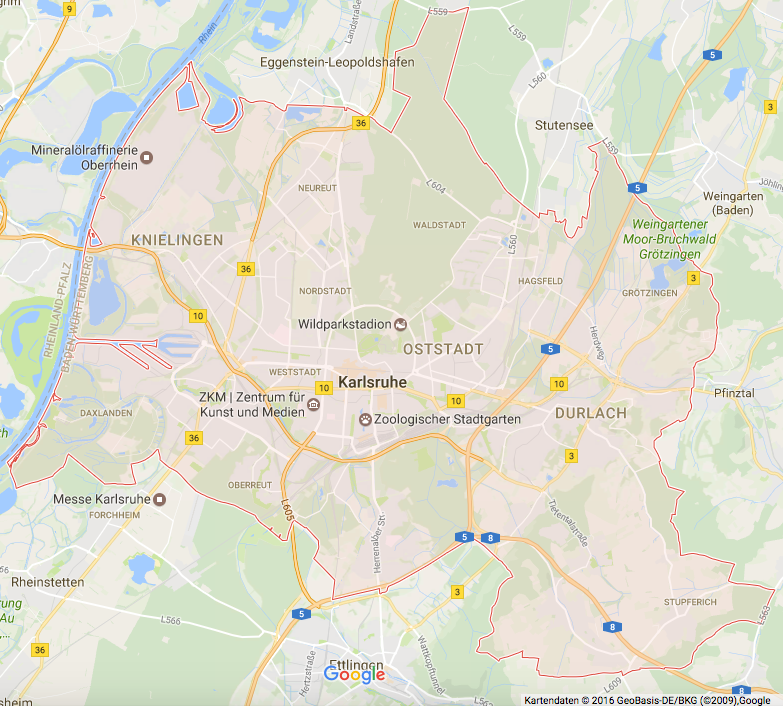
\includegraphics[width=0.55\textwidth]{images/3_Stadtgebiet_KA_zoom12.png}
    \caption{Darstellung der Gemarkungsgrenze des Stadtkreises Karlsruhe [Quelle: google maps, Zoomstufe 12]}
    \label{fig:Stadtgebiet_KA}
\end{figure}
%
\begin{figure}
  \centering
    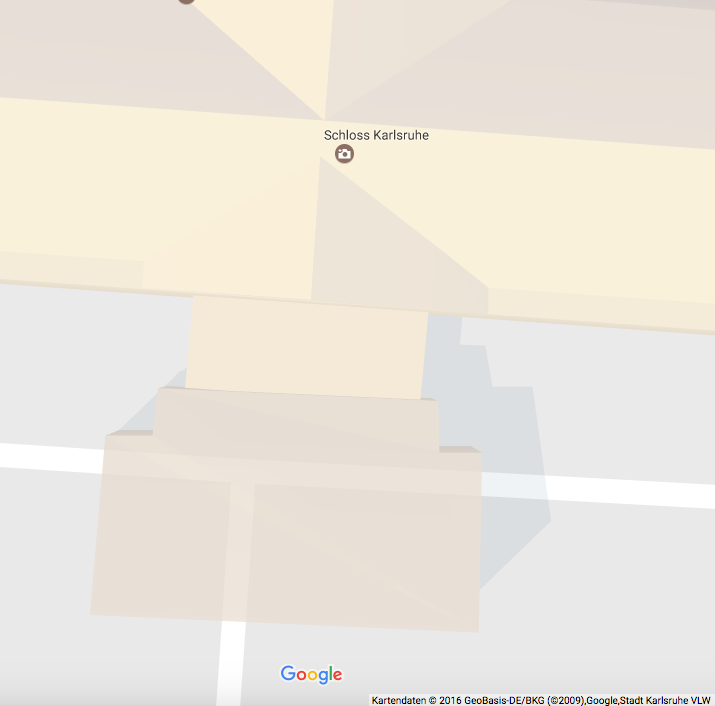
\includegraphics[width=0.6\textwidth]{images/3_KA_Schloss_zoom21.png}
    \caption{Darstellung des Karlsruher Schlosses bei höchster verfügbarer Zoomstufe [Quelle: google maps, Zoomstufe 21]}
    \label{fig:Schloss_KA}
\end{figure}
%
Da google maps die wählbaren Zoomstufen nicht mit einem festen kartographischen Maßstab verknüpft, muss dieser durch eigene Abstandsmessungen ermittelt werden. Bei Zoomstufe 17 besitzt eine der erzeugten quadratischen Einzelkacheln beispielsweise eine Kantenlänge von ca. \num{500} \si{\metre}, wie in Abbildung \ref{fig:Zoomvgl} zu sehen ist.\\
%
\begin{figure}
  \centering
    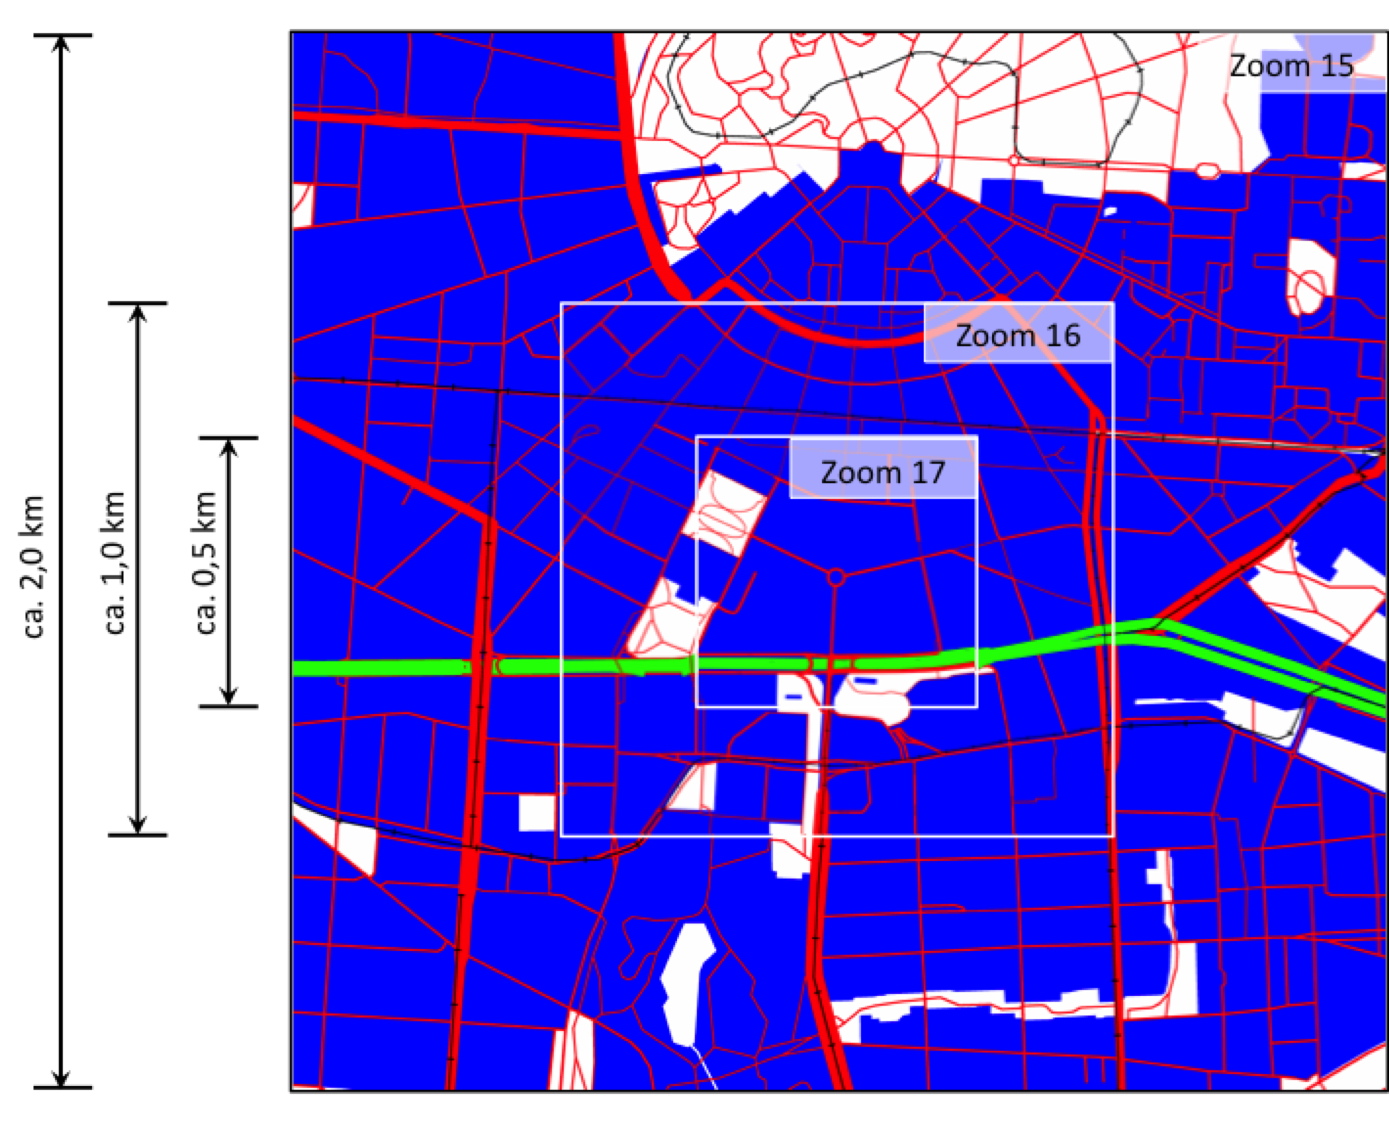
\includegraphics[width=0.6\textwidth]{images/3_Zoomvergleich_KA.png}
    \caption{Vergleich der Kachelabmessungen bei verschiedenen Zoomstufen}
    \label{fig:Zoomvgl}
\end{figure}
%
%
\newline
\begin{figure}
  \centering
    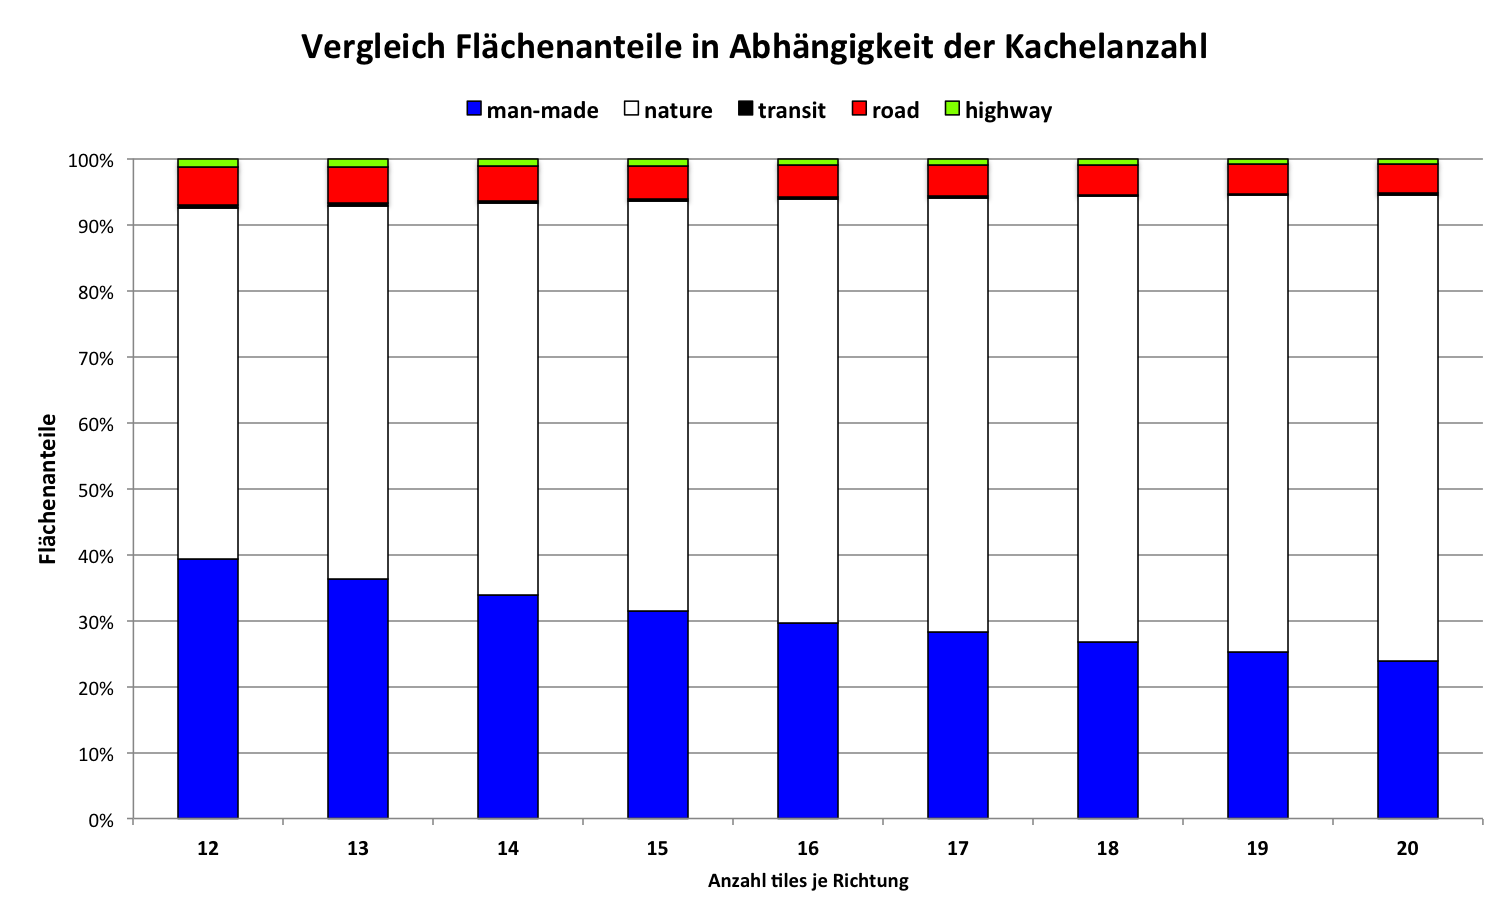
\includegraphics[width=0.92\textwidth]{images/3_Kachelvergleich_KA.png}
    \caption{Ergebnisse der Flächenanalyse für den Stadtkreis Karlsruhe für verschiedene Kachelanzahlen}
    \label{fig:Kachel_vgl}
\end{figure}
%
Im Weiteren wird die Flächenanalyse nun für verschiedene Anzahlen an Kacheln durchgeführt, um zu untersuchen, wie sich die Flächenanteile mit zunehmendem Einzugsgebiet der Analyse verändern. Die Ergebnisse der Flächenanalyse für die Eingabe an Tiles je Richtung zwischen 12 und 20 ist in Abbildung \ref{fig:Kachel_vgl} dargestellt.\\
Mit steigender Kachelzahl wird immer mehr des Stadtrandes und des Umlandes in die Analyse einbezogen, die Anteile von Verkehrsflächen und \textit{man-made area} an der Gesamtfläche sinken ab zu Gunsten der Naturflächen, welche bei  \((n:=15)\) (Kantenlänge des Analysequadrates ca. \num{14.5} \si{\kilo\metre}) und  \((n:=16)\) (Kantenlänge des Analysequadrates ca. \num{15.5} \si{\kilo\metre}) mehr als \num{60} \% einnehmen. Die zuletzt erwähnten Kachelanzahlen erzeugen ein Analysequadrat, welches in seinen Ausdehnungen in der Größenordnung des Stadtgebiets liegt. Für eine vollkommene Umschließung des Stadtgebiets (maximale Nord-Süd-Ausdehnung ca. \num{16.5} \si{\kilo\metre}), maximale Ost-West-Ausdehnung ca. \num{19.0} \si{\kilo\metre}) muss für die Anzahl an Kacheln \((n:=20)\) gewählt werden.\\
\newline
Allerdings muss erwähnt werden, dass die in Abbildung \ref{fig:Stadtgebiet_KA} dargestellte Gemarkung durch eine solche quadratische Analysefläche nur unzureichend angenähert werden kann. Dies zeigt ein Vergleich der Analyseergebnisse mit den Werten des Statistischen Landesamtes: hier wird der Anteil von Naturflächen mit ca. \num{52} \% angegeben, während die Analyse ca. \num{70} \% berechnet. Diese Überschätzung kann darauf zurückgeführt werden, dass bestimmte Bereiche wie beispielsweise große natürliche und landwirtschaftliche Bereiche in der Analyse erscheinen, obwohl sie nicht zum Stadtgebiet Karlsruhe gehören.\\
%
\begin{figure}
  \centering
    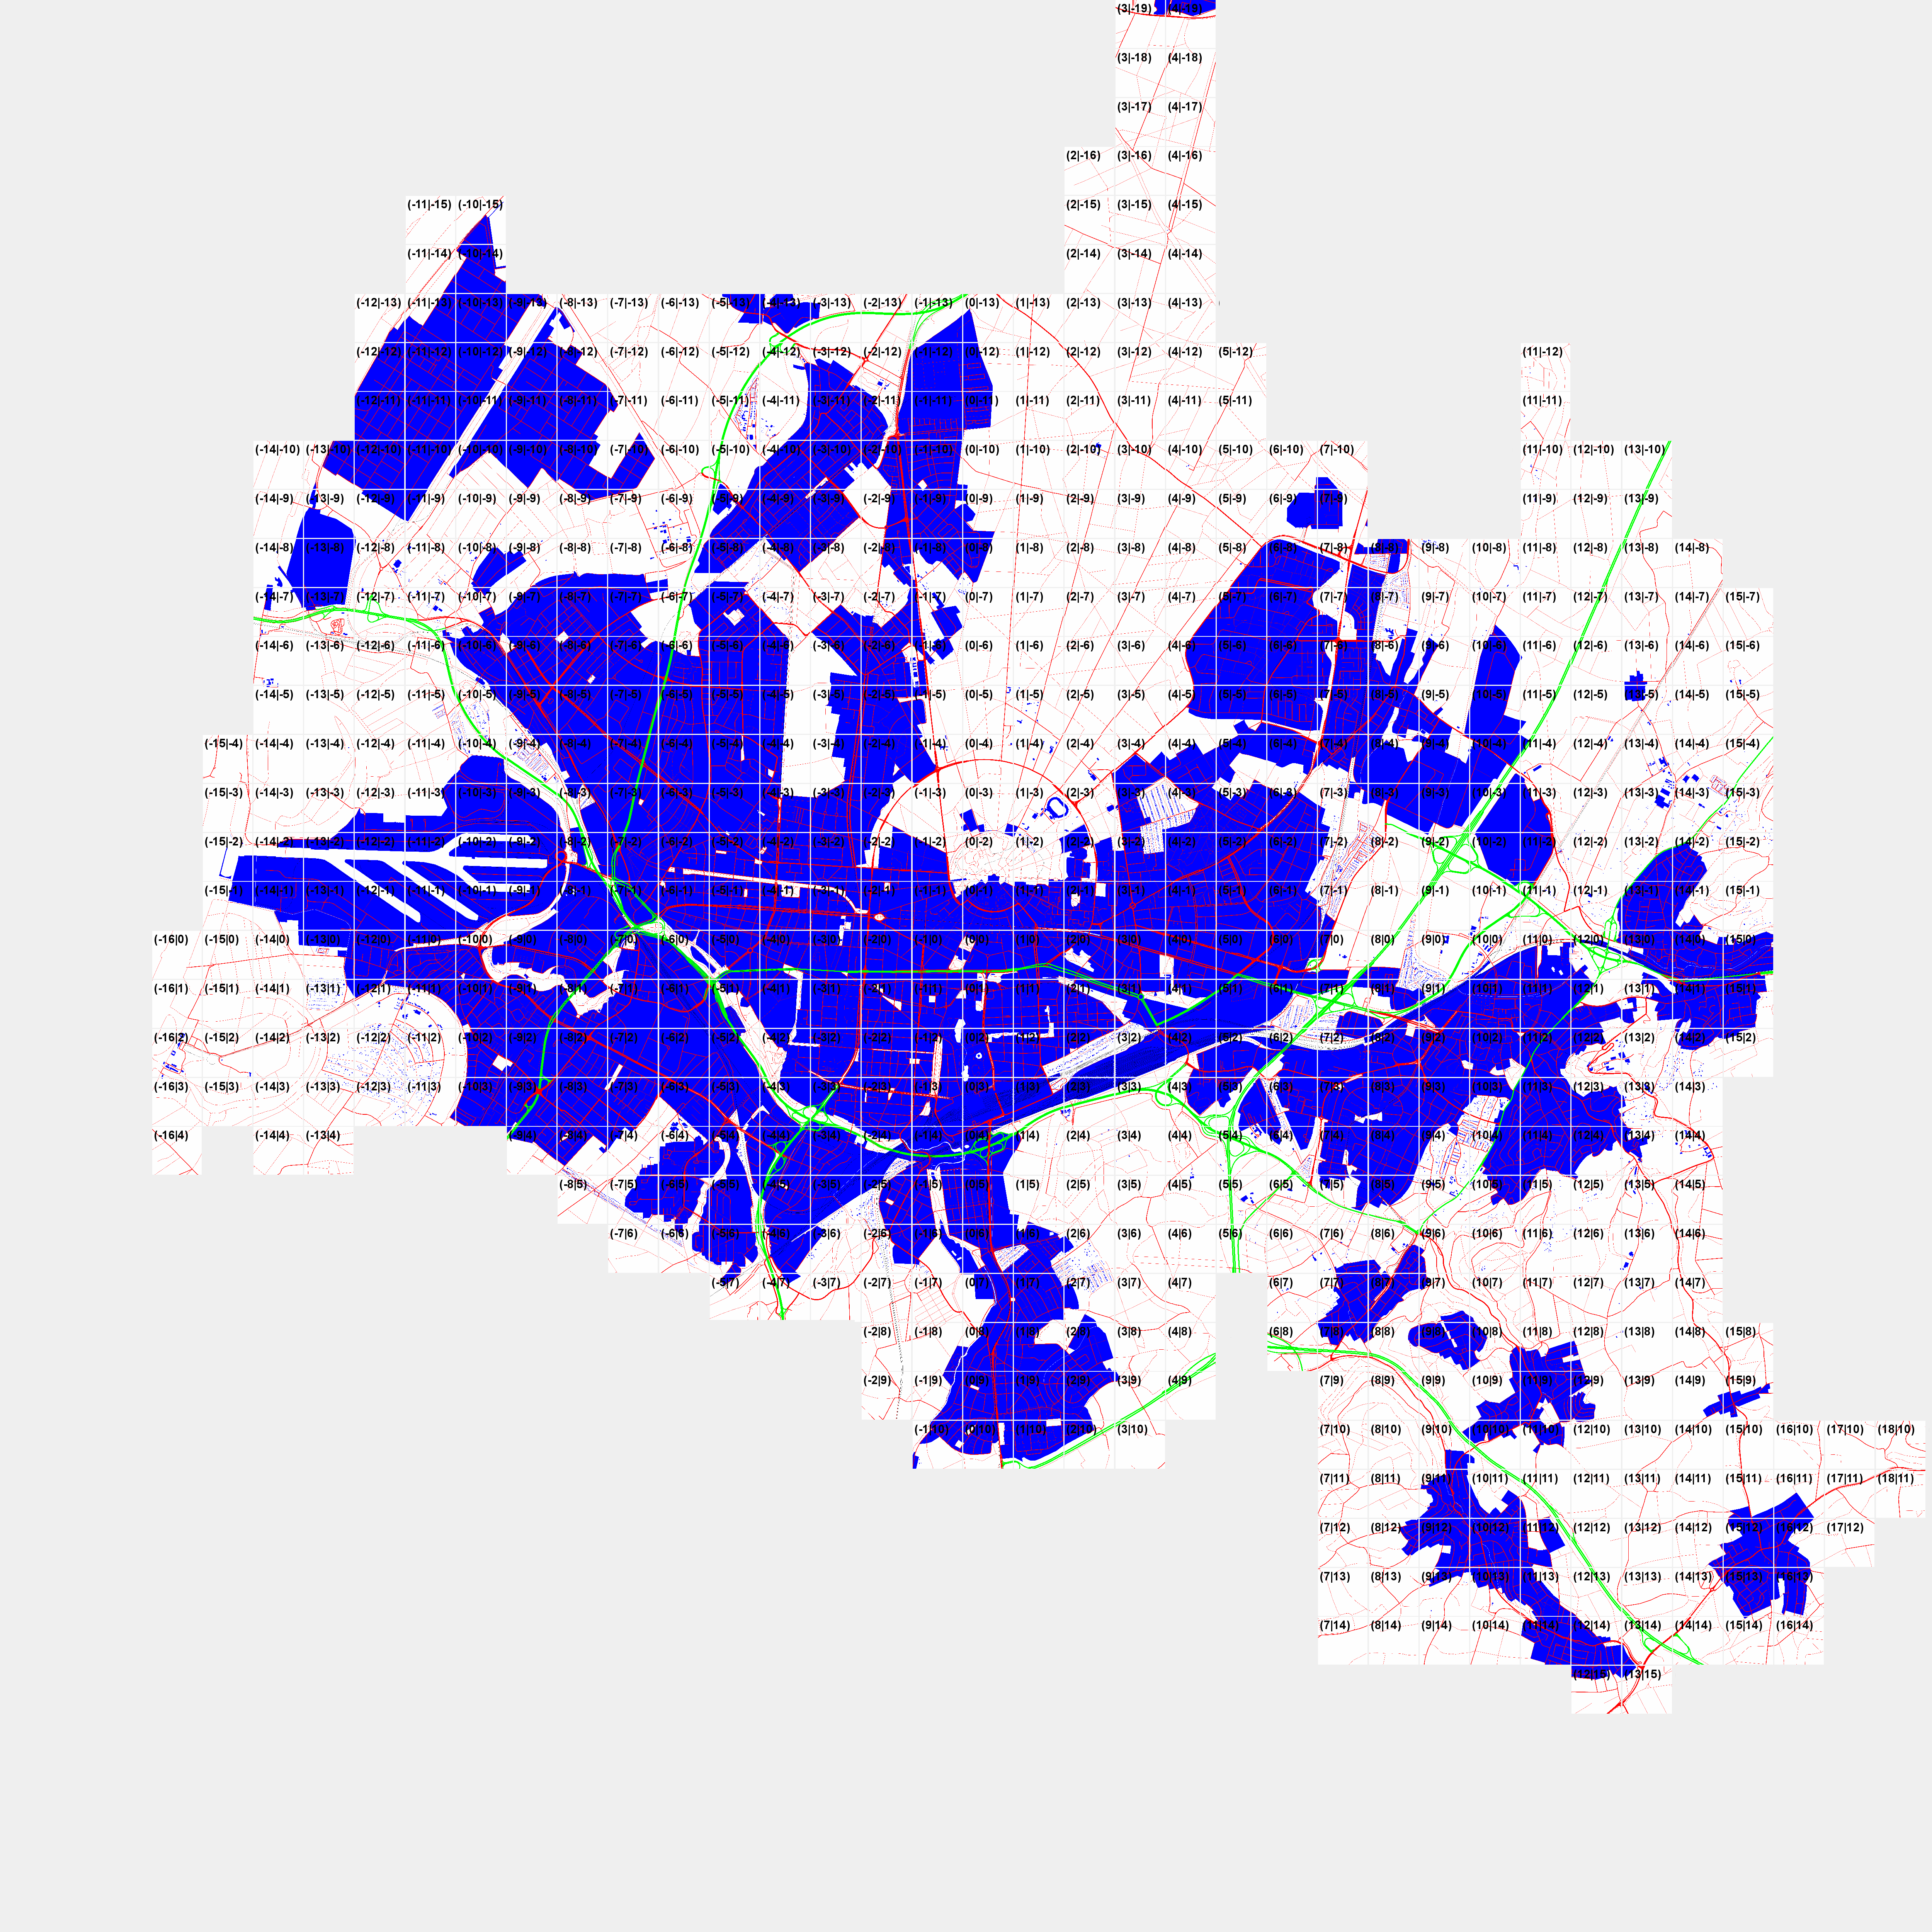
\includegraphics[width=0.9\textwidth]{images/3_KA_Kacheln_skip_ohne_zahlen.png}
    \caption{Darstellung der ausgewählten Kacheln zur genaueren Approximation der Karlsruher Stadtgrenze}
    \label{fig:Karlsruhe_skip_tiles}
\end{figure}
%
%
\begin{figure}
  \centering
    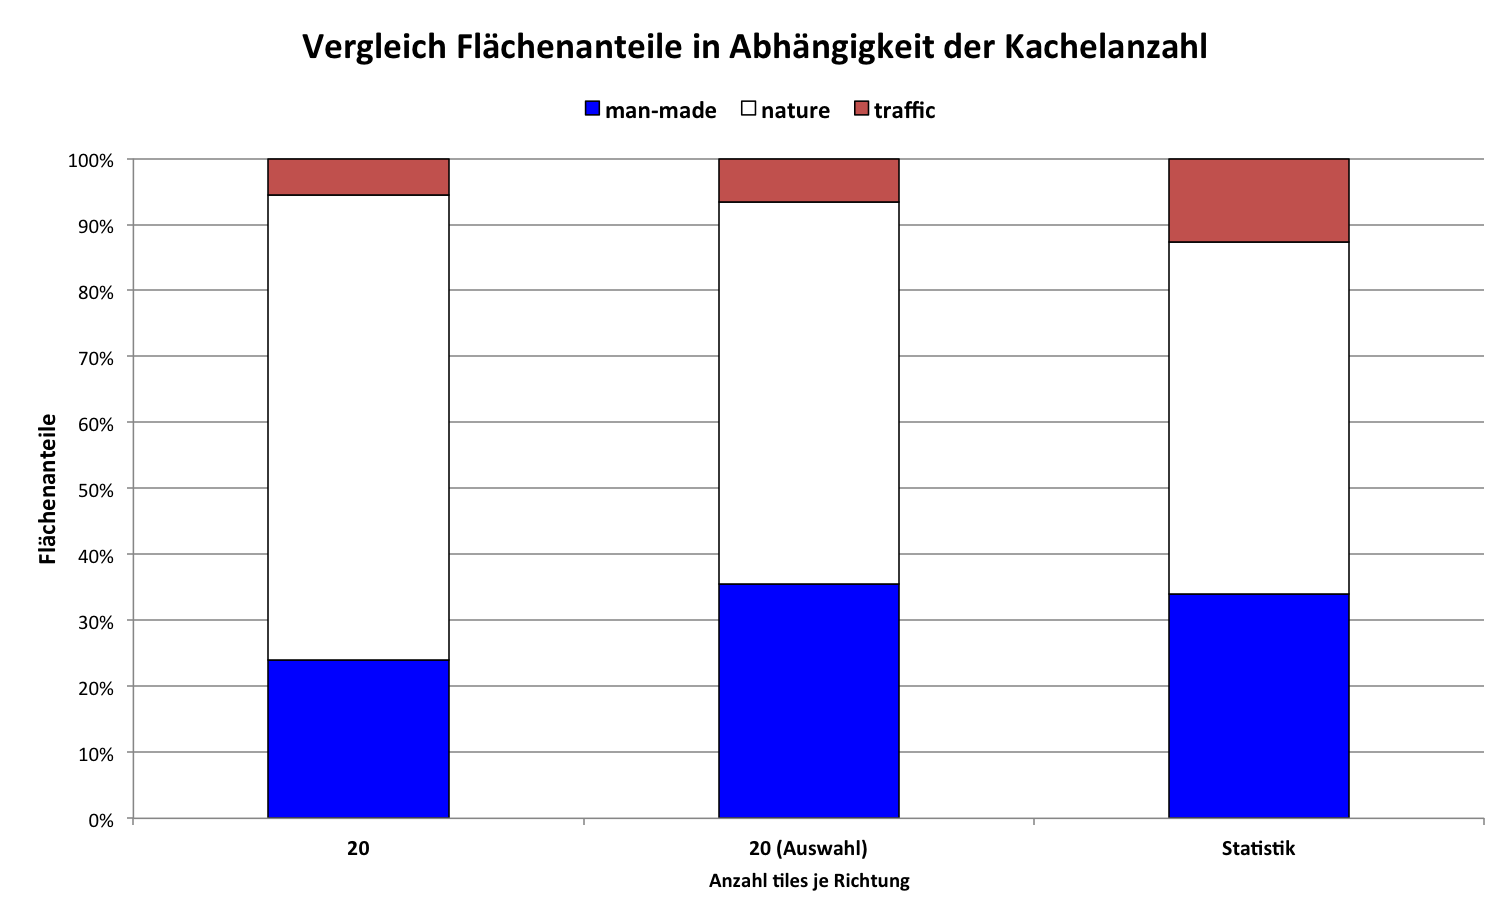
\includegraphics[width=0.92\textwidth]{images/3_Kachelvergleich_KA_skip.png}
    \caption{Ergebnisse der Flächenanalyse für den Stadtkreis Karlsruhe mit und ohne Kachelauswahl im Vergleich zu den statistischen Daten}
    \label{fig:Kachel_skip_vgl}
\end{figure}
%
%
\begin{figure}
  \centering
    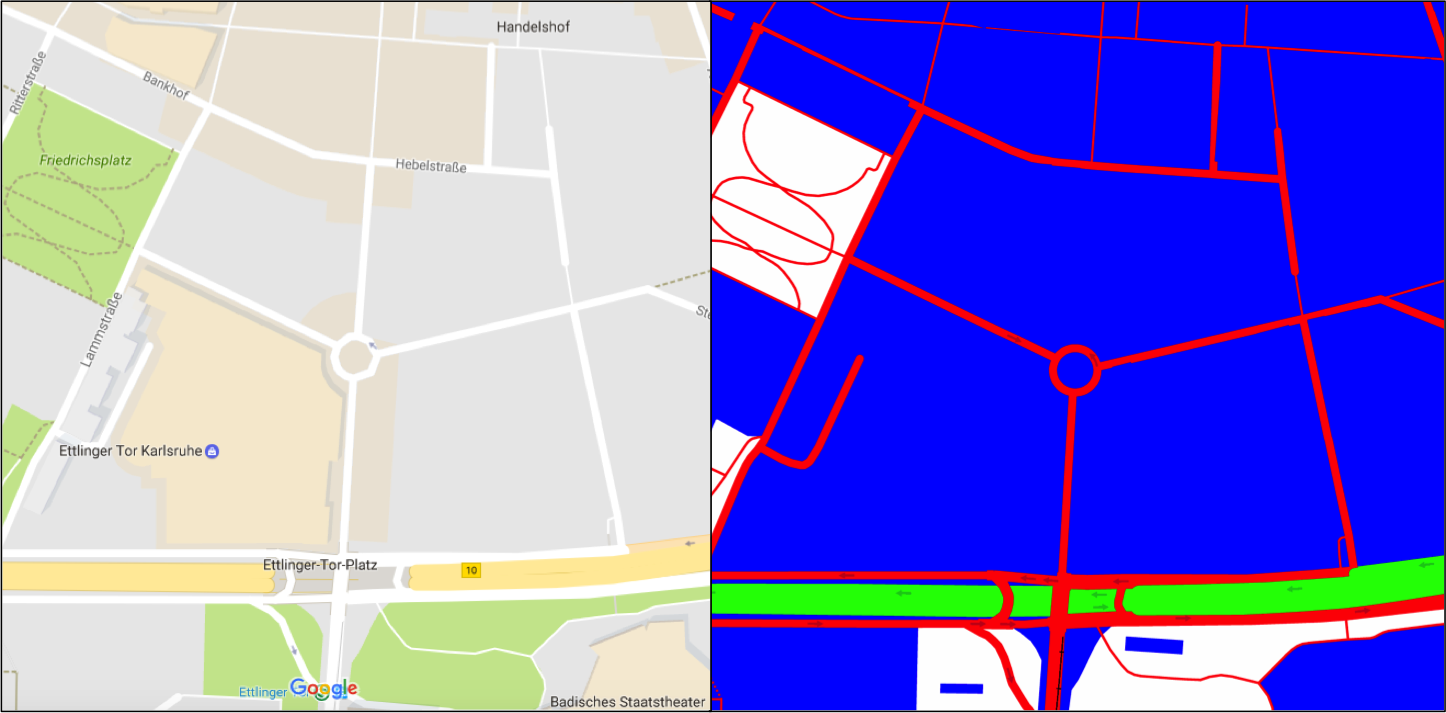
\includegraphics[width=0.85\textwidth]{images/3_google_Einstufung_Nutzung.png}
    \caption{Darstellung einer Straße in der Web-Ansicht (links) und Einstufung als man-made area nach dem Download (rechts)}
    \label{fig:versch_nutz_einstuf}
\end{figure}
%
Eine bessere Approximation kann durch gezielte Auswahl bzw. gezieltes Ausschließen einzelner Kacheln erreicht werden. Im Folgenden werden daher aus der Berechnung, die auf einer Kachelanzahl \((n:=20)\) basiert, diejenigen Kacheln ausgeschlossen, die außerhalb des Stadtgebietes liegen, sodass die übrigen die Stadtgrenze bestmöglich approximieren. Eine Darstellung der gewählten Kacheln findet sich in Abbildung \ref{fig:Karlsruhe_skip_tiles}. Dadurch verringert sich die Gesamtzahl der analysierten Kacheln von  ursprünglich \(1521\) auf nun \(680\). Das Resultat der Berechnung mit selektiertem Analysegebiet ist in Abbildung \ref{fig:Kachel_skip_vgl} den Ergebnissen der Berechnung mit vollen \(1521\) Kacheln sowie den aufbereiteten Daten des Landesamtes gegenübergestellt. Hierbei ist zu beachten, dass im Gegensatz zur bisherigen Benennung die Kategorien \textit{roads}, \textit{highway} sowie \textit{transit} in dieser Darstellung zur Oberkategorie \textit{traffic} zusammengefasst wurden, um eine Vergleichbarkeit der Berechnungsergebnisse mit den statisitschen Daten, welche einer anderen Klassifizierung folgen, zu ermöglichen. Während die Flächenanteile der Kategorie \textit{man-made} in der Berechnung um weniger als  \num{2} \% von denen des statistischen Landesamtes abweichen, zeigt sich bei Verkehrsflächen respektive Naturflächen eine Abweichung von rund \num{5} bis \num{6} \%. Letzteres kann unter anderem auf die unterschiedlichen Einstufungen der Flächen als Siedlungs- oder als Verkehrsfläche zurückgeführt werden. Ein Beispiel hierfür ist der Bereich um das Ettlinger Tor in Karlsruhe, der in Abbildung \ref{fig:versch_nutz_einstuf} dargestellt ist: Während in der Webansicht von google maps (links) in Kachelmitte eine in Nord-Süd-Richtung verlaufende Straße zu erkennen ist, wird diese von google tatsächlich, wie sich bei der Analyse (rechts) zeigt, als \textit{man-made area} eingestuft.\\

% b) Leitfaden zur Verkehrsanalyse
\subsection{Leitfaden zur Verkehrsanalyse}
Nachdem anhand des Beispiels Karlsruhe gezeigt worden ist, dass das entwickelte Verfahren zur Flächenanalyse die tatsächliche Flächennutzungen sehr gut darstellen kann, soll dessen Anwendung im weiteren Verlauf der Untersuchung bei einer Auswahl von Städten durchgeführt werden.\\
\newline
Das im Folgenden beschriebene Vorgehen stellt eine allgemeine Empfehlung für den Aufbau einer Verkehrsanalyse dar. Dessen Anwendung wird im Einzelfall sowohl von der Stadtgeometrie bzw. der Topograhpie der Region als auch von der Fragestellung bzw. Zielsetzung der Untersuchung maßgeblich beeinflusst. Daher ist es zielführend, vor Anwendung des folgenden Schemas in einer kurzen Voruntersuchung das Untersuchungsgebiet festzulegen und die gewünschten Zielgrößen zu definieren.
\begin{enumerate}
\item \textbf{Festlegen des Zentrums für die Kachelauswahl:} Im ersten Schritt muss ein geographischer Punkt als Zentrum für die Kachelauswahl gewählt werden. Dies kann der (zentrale) Punkt sein, den die Web-Anwendung google maps bei Eingabe des Stadtnames im Suchfeld ausgibt. In vielen Fällen ist es aber sinnvoller, den Punkt unabhängig davon möglichst mittig im bestimmten  Untersuchungsgebiet zu wählen, um die Anzahl an Kacheln, die zur vollständigen Überdeckung des Untersuchungsgebietes notwendig sind, gering zu halten. In speziellen Fällen, in denen beispielweise nur ein kurzer Streckenabschnitt zu analysieren ist, muss der zentrale Punkt ohnehin frei gesetzt werden. Die Koordinaten des Punktes sind im Format (\textit{latitude}, \textit{longitude}) anzugeben.
%
\begin{figure}
  \centering
    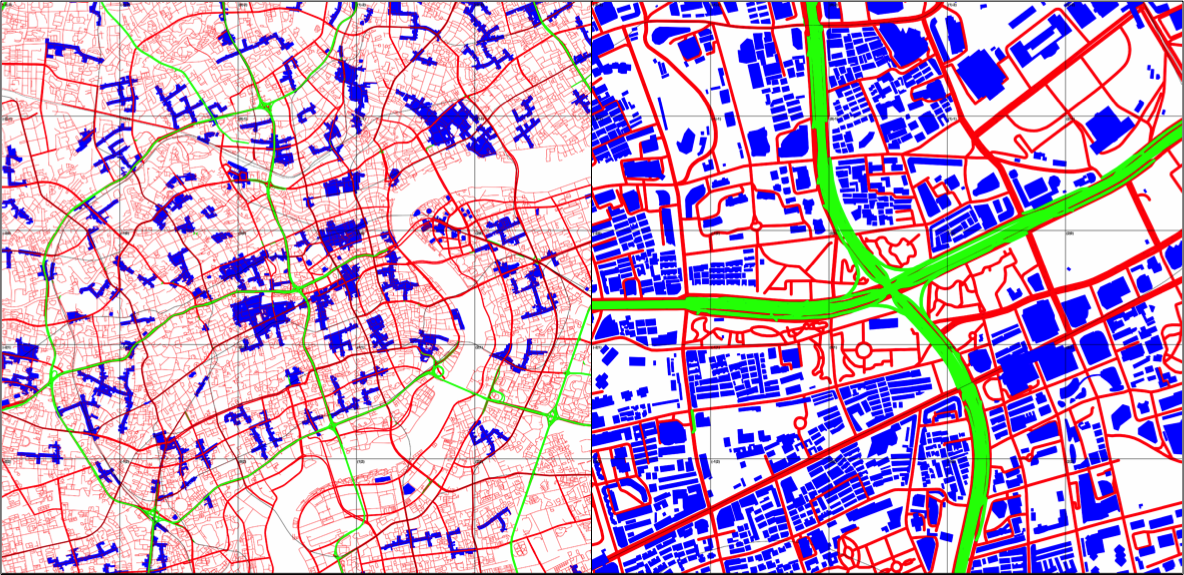
\includegraphics[width=0.92\textwidth]{images/3_Shanghai_Problem_Datenaufloesung}
    \caption{Darstellung des Stadtzentrums von Shanghai bei Zoomstufe 15 (links) und 18 (rechts); (links Darstellungsfehler aufgrund sehr detaillierter Gebäudeumrisse)}
    \label{fig:Fehler_Shanghai}
\end{figure}
%
%
\begin{figure}
  \centering
    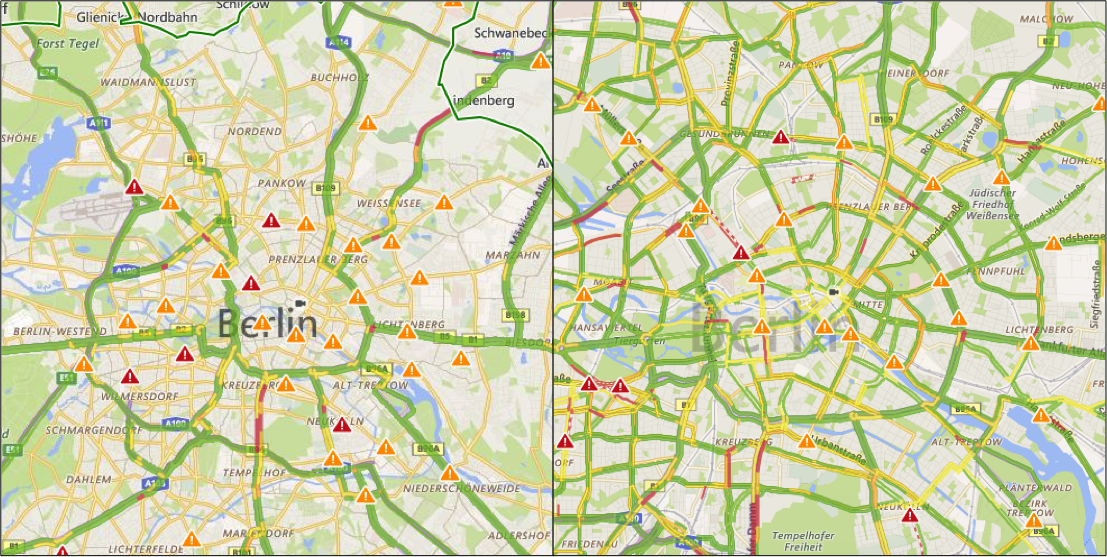
\includegraphics[width=0.92\textwidth]{images/3_bing_Aufloesung_traffic}
    \caption{Darstellung des Stadtzentrums von Berlin in verschiedenen Zoomstufen zeigt das Straßennetz in verschiedener Detaillierung}
    \label{fig:Fehler_Berlin}
\end{figure}
%
\item \textbf{Festlegen der Zoomstufe:} Im zweiten Schritt muss die Zoomstufe für die Kacheln festgelegt werden. Wie oben bereits beschrieben wurde, gilt es hierbei zwischen der Auflösegenauigkeit und dem steigenden Rechenaufwand abzuwägen. Daneben kann aber auch die lokal vorliegende Datengrundlage einen entsprechenden Einfluss auf die mögliche Zoomstufe besitzen. Bei den Flächendaten einerseits zeigt sich bei sehr präzisen Geodaten, dass google maps bei zu niedriger Zoomstufe die hochaufgelösten Daten zum Teil nicht mehr ordnungsgemäß abbilden kann und aus diesem Grund die bebauten Flächen falsch zuordnet. Ein Beispiel hierfür ist in Abbildung \ref{fig:Fehler_Shanghai} zu sehen: das Zentrum von Shanghai wird bei Zoomstufe 15 zu weiten Teilen als Naturfläche (Farbe weiß) eingestuft, die Gebäudeumrisse werden erst bei Zoomstufe 18 deutlich. Andererseits zeigt sich, dass bei den Verkehrsdaten kleinere Straßen bei zu niedriger Zoomstufe nicht dargestellt werden, obwohl sie mit Verkehrsinformationen belegt sind. Dies ist am Beispiel des Stadtzentrums von Berlin in Abbildung \ref{fig:Fehler_Berlin} dargestellt. Um die beiden genannten Probleme zu vermeiden empfiehlt es sich, verschiedene Zoomstufen im Hinblick auf deren Auflösegenauigkeit und ggf. auftretende Fehldarstellungen zu testen und die erzeugten Resultate zu vergleichen.
%
\item \textbf{Einstellung Anzahl Tiles:} Im folgenden Schritt wird die Anzahl der Tiles ausgewählt. Hierbei ist im Wesentlichen darauf zu achten, dass einerseits das Untersuchungsgebiet durch das Kachelraster vollständig abgedeckt wird, gleichzeitig aber die Gesamtzahl möglichst begrenzt bleibt. Kann hierbei kein zufrieden stellender Kompromiss zwischen beidem erzielt werden, müssen die in den vorhergegangen Schritten festgelegten Werte ggf. geändert werden. Die Begrenzung der Kachelanzahl ist besonders im Falle der Verkehrsdaten von entscheidender Wichtigkeit, da die Downloadraten durch die Anbieter des Kartenmaterials begrenzt sind und so nur eine bestimmte maximale Anzahl an Kacheln je Zeiteinheit analysiert werden kann. Ist die Gesamtzahl der Kacheln zu groß, kann der gewählte Zeitschritt der Analyse unter Umständen nicht mehr eingehalten werden.  
%
\item \textbf{Auswahl zu überspringende Tiles:} Abschließend können noch einzelne Tiles aus der Analyse ausgeschlossen werden. Hierzu zählen unter anderem Bereiche, die entweder keinen Einfluss auf die Analyse besitzen (z. B. reine Naturflächen) oder die im Rahmen der Untersuchung bewusst ausgeklammert werden (z. B. vorbeiführende Fernstraße soll aus der Stadtanalyse ausgeschlossen werden). Hierzu werden die auszuschließenden Kacheln einfach über die Indizes, welche ihren Platz innerhalb des Kachelrasters festlegen, angegeben.
\end{enumerate}




  \newpage
  \section{Verkehrsanalyse}
Der nächste Schritt nach der Auswahl der geographischen Parameter ist die Verkehrsanalyse. In diesem Kapitel sollen im Sinne einer Machbarkeitsstudie Möglichkeiten aufgezeigt werden die Verkehrsdaten zu visualisieren und zu analysieren. Danach werden sie auf eine repräsentative Zahl, also einen \grq Stauindex\grq  reduziert.\\
Das Ziel der Auswertung der Verkehrsdaten ist es die Verkehrssituation in Städten über einen längeren Zeitraum bewerten zu können und eine Vergleichbarkeit zwischen Städten herzustellen. Ein Stauindex kann hier einen einfachen Überblick über die Daten gewährleisten.\\ Zu verkehrlich besonders interessanten oder auffälligen Zeiten bietet es sich an auf die detaillierteren Daten zurückzugreifen um einen besseren Überblick über die Situation zu gewinnen.

\subsection{Aufbau der Verkehrsdaten}
Die Verkehrsdaten werden von Bing Maps durch Einfärben der Straßen in 4 verschiedenen Farben für die verschiedenen Verkehrszustände bereitgestellt. Es gibt die Zustände kein Verkehr (grün), wenig Verkehr (gelb), mittlerer Verkehr (orange) und dichter Verkehr (rot). Abbildung~\ref{fig:farben_einfuehrung} zeigt beispielhaft einen Ausschnitt der Verkehrssituation in Karlsruhe aus Bing Maps. Insbesondere fällt auf, dass Bing Maps für zahlreiche verkehrsrelevante Straßen in Karlsruhe keine Verkehrsinformationen enthält.\\
\begin{figure}
  \centering
    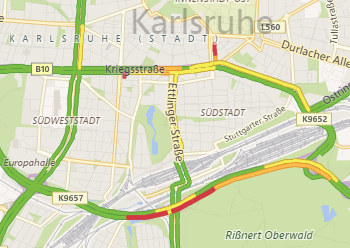
\includegraphics[width=0.7\textwidth]{images/verkehr_einfuehrung.png}
    \caption{Beispielhafte Verkehrsdaten aus Bing Maps. Die Daten repräsentieren die  Verkehrszustände: kein Verkehr (grün), wenig Verkehr (gelb), mittlerer Verkehr (orange) und dichter Verkehr (rot)}
    \label{fig:farben_einfuehrung}
\end{figure}

Die angegebenen Farben sind dabei nur bedingt proportional zur Verkehrsstärke und eher als Beeinflussung der Verkehrssituation, statt als Menge der Fahrzeuge pro Zeiteinheit zu sehen. Abbildung~\ref{fig:uebersicht_verkehrszustaende} zeigt Beispielhaft die Aufnahmen von Verkehrskameras mit den zu der Zeit in Bing Maps angezeigten Verkehrszuständen.\\  
\begin{figure}
\begin{tabular}{@{}cc@{}}
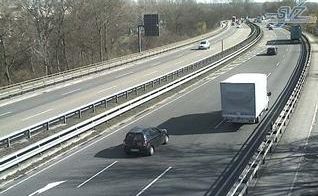
\includegraphics[width = 0.48\textwidth]{images/no_traffic.png} &
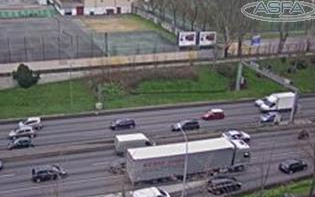
\includegraphics[width = 0.48\textwidth]{images/low_traffic.png} \\ 
\textbf{kein Verkehr}  & \textbf{leichter Verkehr}   \\
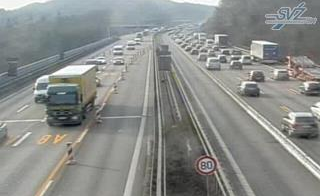
\includegraphics[width = 0.48\textwidth]{images/medium_traffic.png} & 
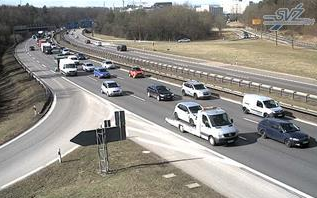
\includegraphics[width = 0.48\textwidth]{images/heavy_traffic.png} \\
\textbf{mittlerer Verkehr} & \textbf{dichter Verkehr}\\
\end{tabular}
\caption{Bilder von Verkehrskameras zu den Verkehrszustände kein Verkehr, leichter verkehr, mittlerer Verkehr und dichter Verkehr aus Bing Maps}
\label{fig:uebersicht_verkehrszustaende}
\end{figure}

Mit der in Kapitel~\ref{chapter:christof} beschriebenen Methode lassen sich die Verkehrsinformationen auslesen und die Anteile der jeweiligen Verkehrszustände an allen Pixeln mit Verkehrsinformation ermitteln.
Eine Möglichkeit die Anteile der Verkehrszustände graphisch anschaulich darzustellen ist als gestapelter Graph.
Abbildung~\ref{fig:stacked_stuttgart} zeigt die Anteile von leichtem, mittlerem, und dichtem verkehr in Stuttgart am Dienstag, dem 06.02.2017. Die Form der summierten Anteile entspricht sehr gut der aus dem Verkehrswesen bekannten Tagesganglinie. 
\begin{figure}
  \centering
    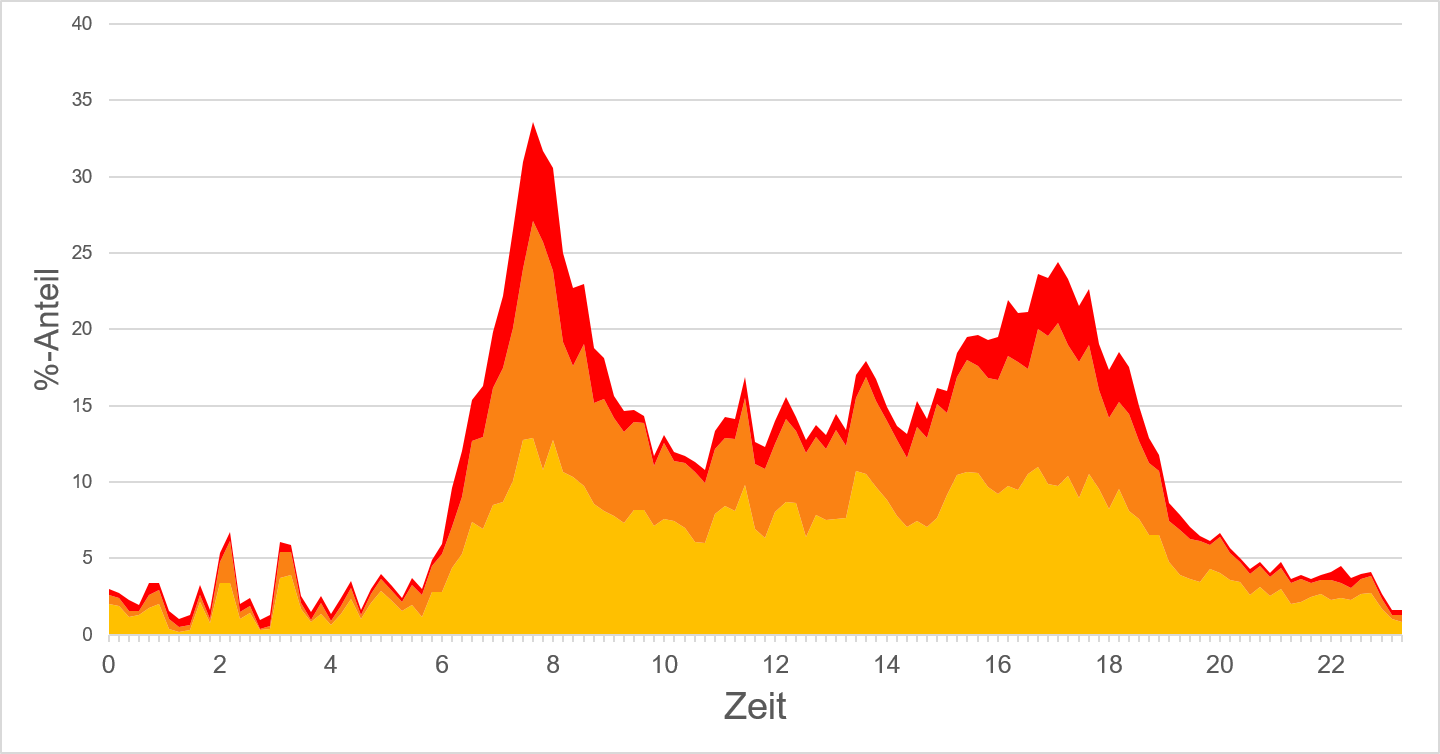
\includegraphics[width=1.0\textwidth]{images/stacked_stuttgart.png}
    \caption{Prozentualer Anteil der Verkehrszustände wenig Verkehr (gelb), mittlerer Verkehr (orange) und dichter Verkehr (rot) an allen Pixel auf dem Kartenausschnitt, die mit Verkehrsinformationen belegt sind.}
    \label{fig:stacked_stuttgart}
\end{figure}

\subsection{Stauindex}

Ausgehend von den Assoziationen mit dem Wort Stauindex lassen sich folgende Anforderungen ableiten:
\begin{itemize}
\item Der Stauindex soll die verschiedenen Verkehrszustände entsprechend ihrer Beeinträchtigung der Verkehrsteilnehmer unterschiedlich stark gewichten.
\item Er soll außerdem Verkehrszuständen mit stärkerer Beeinträchtigung der Verkehrsteilnehmer einen höheren Index zuweisen.
\item Um eine Vergleichbarkeit zwischen Städten  herstellen zu können, soll der Index sich auf die mit Verkehrsinformationen belegte Fläche beziehen. Andernfalls würde der ausgewählte Kartenausschnitt in Kombination mit der Struktur der Stadt eine sehr große Rolle spielen. 
\end{itemize}
Diese Voraussetzungen lassen sich mit folgender Gleichung abbilden:

\begin{equation}\label{eq:1}
\frac{\beta_l\cdot p_{leicht}+\beta_m\cdot p_{mittel}+\beta_d\cdot p_{dicht}}{P_{mit Info}}
\end{equation}
\begin{itemize}
\item $\beta_l$: Gewichtungsfaktor für leichten Verkehr
\item $p_{leicht}$: Anteil an leichtem Verkehr
\item $\beta_m$: Gewichtungsfaktor für mittleren Verkehr
\item $p_{mittel}$: Anteil an mittlerem Verkehr
\item $\beta_d$: Gewichtungsfaktor für dichten Verkehr
\item $p_{dicht}$: Anteil an dichtem Verkehr
\item $p_{mit Info}$: Anteil der mit Verkehrsinformationen belegten Pixeln
\end{itemize}

Bei der Abbildung der Verkehrssituation auf einen Stauindex und der Vergleichbarkeit zwischen Städten treten mehrere Probleme auf. Zum einen wird die Verkehrssituation in verschiedenen Städten aufgrund der unterschiedlichen Datenverfügbarkeit von Bing Maps unterschiedlich dargestellt. Große Städte wie Berlin verfügen oft über sehr umfangreiche Verkehrsinformationen. In kleinen und mittelgroßen Städten sind i.d.R. nur Verkehrsinformationen für die größten Straßen verfügbar, während andere verkehrlich relevante Straßen über keine Informationen verfügen.\\ Der Mangel an Informationen deutet in erster Linie auf wenig Verkehrsteilnehmer und somit eine gute Verkehrssituation hin. Jedoch können die Gründe hierfür auch in den von Bing Maps verwendeten Algorithmen oder einem geringen Smartphonebesitz liegen. Dies führt zu einer schlechteren Darstellung der Verkehrssituation in kleinen und mittelgroßen Städten, da der guten Verkehrssituation auf verkehrlich relevanten Straßen nicht Rechnung getragen wird.\\  
Eine Möglichkeit dieses Problem zu beheben besteht darin, die aus Google Maps ermittelte gesamte Straßenfläche einer Stadt mit einem Gewichtungsfaktor einzubeziehen. Dabei bleibt jedoch die Frage offen, welcher Anteil der Straßen einer Stadt als verkehrlich relevant anzusehen ist.\\
Ein weiteres Problem besteht zu Schwachlastzeiten, wenn besondere Verkehrsbeeinträchtigungen eintreten. Zu diesen Zeiten sind aufgrund der geringen Anzahl an Verkehrsteilnehmern weniger Straßen mit Verkehrsinformationen belegt. Dieser Zustand ist in Abbildung~\ref{fig:stauindex_problem} beispielhaft dargestellt. 

\begin{figure}
  \centering
    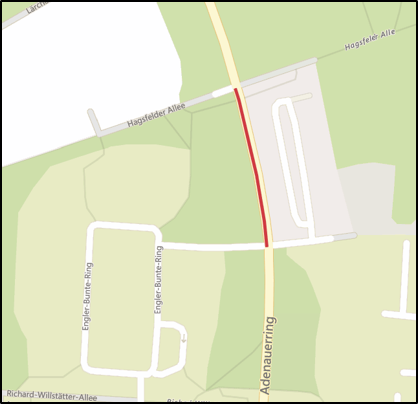
\includegraphics[width=0.5\textwidth]{images/stauindex_problem.png}
    \caption{Problematische Situation bei Berechnung des Stauindex ohne Betrachtung des gesamten Straßenfläche. Diese Situation würde aufgrund der hohen Anzahl an Pixeln mit dichter Verkehrssituation bei insgesamt geringer Verfügbarkeit von Verkehrsinformationen zu einem sehr hohen Stauindex führen.}
    \label{fig:stauindex_problem}
\end{figure}

Ist nun ein Teil der Straßen z.B. durch eine Baustelle oder einen Unfall mit einem mittleren oder dichten Verkehrszustand belegt, führt dies mit Gleichung~\ref{eq:1} zu einem besondere hohen Stauindex. In diesem Fall kann ebenfalls auf die gesamte Straßenfläche zurückgegriffen werden, um den Stauindex zu reduzieren.
Der Stauindex kann auf folgende Weise modifiziert werden, im die gesamte Straßenfläche zu beachten.

\begin{equation}\label{eq:2}
\frac{\beta_l\cdot p_{leicht}+\beta_m\cdot p_{mittel}+\beta_d\cdot p_{dicht}}{P_{mit Info} + \beta_o\cdot P_{ohne Info}}
\end{equation}

\begin{itemize}
\item $\beta_o$: Gewichtungsfaktor für Straßen ohne Verkehrsinformation
\item $p_{ohne Info}$: Anteil der Straßen ohne Verkehrsinformation
\end{itemize}

Die Ergebnisse von Gleichung~\ref{eq:2} sind am Beispiel eines Dienstags in Stuttgart in Abbildung~\ref{fig:stauindex_stuttgart} dargestellt. Hier zeigt sich ebenfalls die bekannte Form der Tagesganglinie. Die Höhe der Morgen- und Abendspitze hängt aufgrund der hohen Anteile von mittlererm und dichtem verkehr stark von der Wahl der Gewichtungsfaktoren ab.\\

\begin{figure}
  \centering
    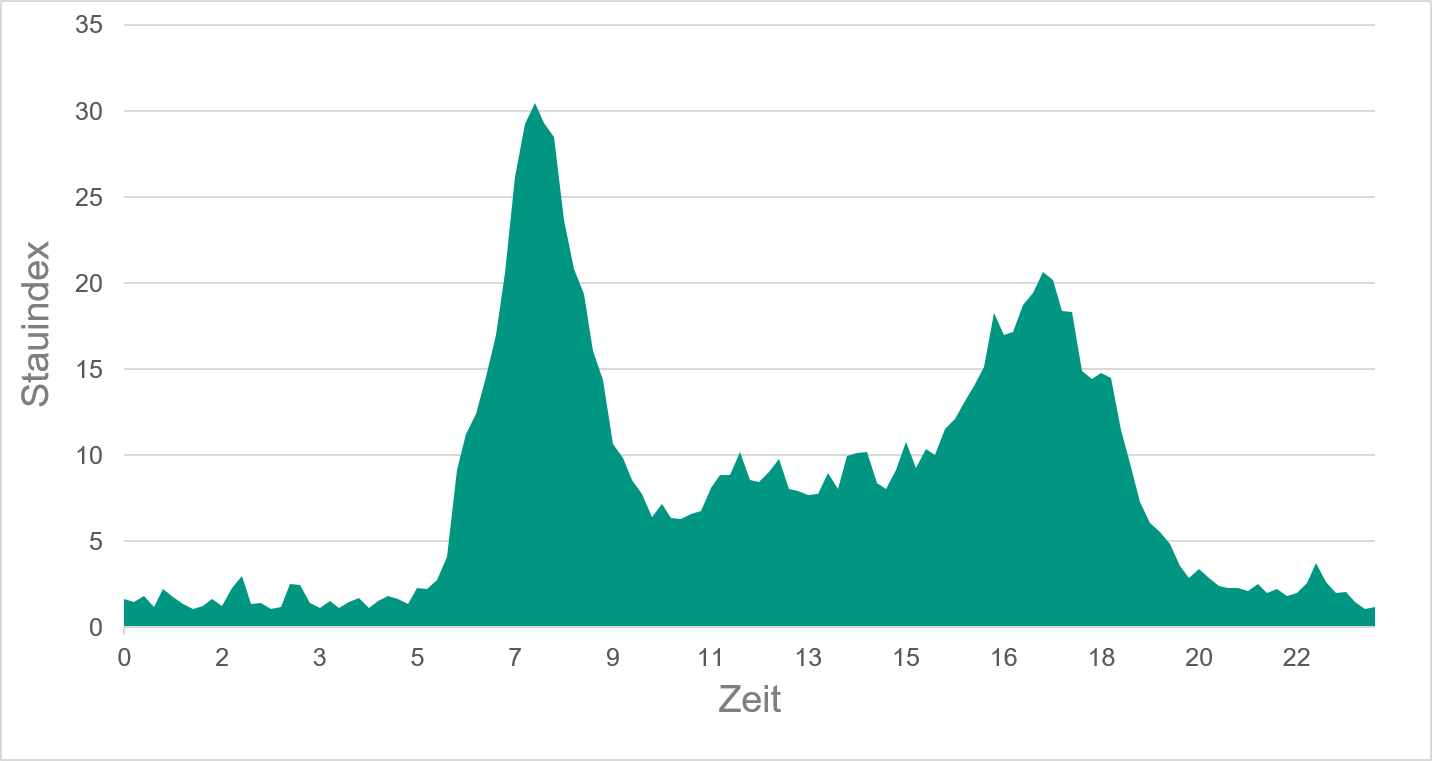
\includegraphics[width=1.0\textwidth]{images/stauindex.png}
    \caption{Stauindex der Stadt Stuttgart während eines Dienstag über einen Zeitraum von 24 Stunden in 10-Minuten-Intervallen aufgenommen.}
    \label{fig:stauindex_stuttgart}
\end{figure}

Der Stauindex bezieht sich bislang nur auf einen Zeitpunkt. Im Sinne eines übersichtlichen Index soll jedoch der Gesamtverkehrssituation über einen längeren Zeitraum ein Index zugeordnet werden. Hierfür bestehen mehrere Möglichkeiten den Index zeitlich zu mitteln. Eine Möglichkeit besteht darin, den arithmetischen Mittelwert über den gesamten Zeitraum zu bilden.\\ Dies hat den Vorteil, dass besondere Verkehrszustände, welche i.d.R nicht den ganzen Tag über anhalten, weniger stark gewichtet werden. Somit ist ein repräsentatives Ergebnis bereits bei geringer Datenverfügbarkeit möglich.
Nachteil dieser Methode ist, dass die Verkehrssituation des ganzen Tages berücksichtigt wird, wobei aber i.d.R. nur die morgendliche und abendliche Hauptverkehrszeit zu wesentlichen Beeinträchtigungen führt.\\ Qualitative Untersuchungen der gesammelten Daten zeigen, dass die Zustände mittlerer- und dichter Verkehr nur während der Hauptverkehrszeit in wesentlichen Mengen auftreten und auf einer Basis des Zustands leichter Verkehr aufsetzen, der während des Tages relativ konstant bleibt und nur in den Schwachlastzeiten abfällt (siehe Abbildung~\ref{fig:stacked_stuttgart}). Diese Basis an leichtem Verkehr kann bei entsprechender Wahl der Gewichtungsfaktoren den Stauindex stark negativ beeinflussen, was dem Prinzip eines Stauindex widersprechen würde. Dieses Problem tritt insbesondere in großen Städten mit hoher Verfügbarkeit an Verkehrsdaten auf.\\ Alternativ zum arithmetischen Mittelwert des Tages ist es auch möglich einen Hauptverkehrszeit-Stauindex zu bilden. Hierfür wird das arithmetische Mittel über eine festzulegende Anzahl an Maximalwerten pro Tag gebildet. Dies löst das diskutierte Problem des des leichten Verkehrs und es wird die Verkehrssituation einer Stadt zur verkehrlich relevante Zeit betrachtet. Die Anfälligkeit gegenüber besonderen Verkehrsereignissen, wie z.B. Staus, steigt jedoch stark an und es ist somit eine wesentlich größere Datenbasis erforderlich. \\


Tabelle~\ref{fig:index_tabelle} zeigt das arithmetische Mittel des ganzen Tages, das Maximum und das Minimum zwischen 8 und 20 Uhr des Stauindex für ausgewählte Städte. Der Index wurde mit Gleichung~\ref{eq:2} berechnet, als Datenbasis wurde ein Zeitraum von 24 Stunden während eines Dienstag verwendet. Die Ergebnisse sind somit nicht repräsentativ für die jeweiligen Städte, zeigen aber aufgrund der Ähnlichkeit, dass es mit weiteren Untersuchungen der Gewichtungsfaktoren und der Kartenausschnitte und einer wesentlich größeren Datenbasis möglich sein könnte eine Vergleichbarkeit der Städte herzustellen.





\begin{figure}
  \centering
    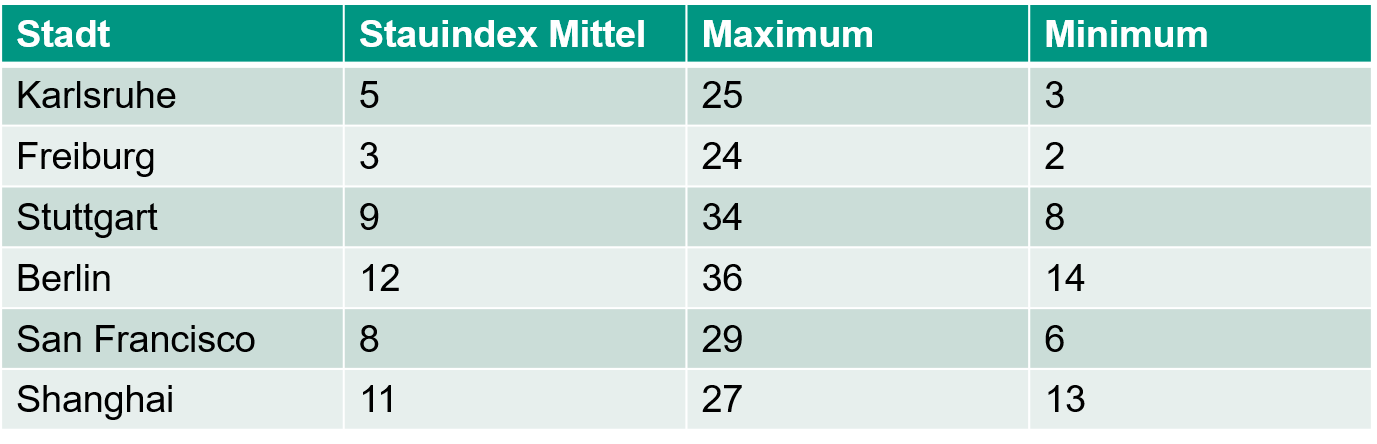
\includegraphics[width=1.0\textwidth]{images/index_tabelle.png}
    \caption{Arithmetisches Mittel des ganzen Tages, Maximum und Minimum zwischen 8 und 20 Uhr des Stauindex für ausgewählte Städte auf Datenbasis eines Dienstages.}
    \label{fig:index_tabelle}
\end{figure}
  \newpage
  \section{Fazit und Ausblick}

Diese Arbeit beschreibt die Entwicklung eines Programms zum Auslesen der Verkehrszustände in BingMaps und der Bodenbedeckungsdaten in GoogleMaps, sowie deren Analyse und Integration in einen Stauindex.\\
Das Programm liest erfolgreich auf Basis eines anzugebenden Mittelpunktes, der Zoomstufe und der Anzahl an Kachellagen um den Mittelpunkt die Anzahl der Pixel aus, die mit den jeweiligen Verkehrszuständen bzw. Bodenbedeckungsdaten belegt sind.\\
Weiterhin wird eine Möglichkeit aufgezeigt, diese Daten in einen Stauindex zu integrieren und diesen zeitlich zu mitteln. Auch wenn die Ergebnisse auf eine mögliche Vergleichbarkeit Stauindizes verschiedener Städte hindeuten, ist jedoch eine tiefergehende Untersuchung und insbesondere eine größere Datenbasis erforderlich, um diese Frage abschließend zu beantworten. Hierzu sollten möglichst viele Städte mit unterschiedlichem Verkehrsfluss in die Untersuchung einbezogen werden, um eine wirkungsvolle Kalibrierung durchführen zu können. Es wird hierbei explizit darauf hingewiesen, dass es nicht zwingend notwendig oder sinnvoll sein muss, einen einzelnen Paramatersatz für alle Städte zu entwickeln. Es sollte stattdessen vielmehr geprüft werden, ob eine Klassifizerung oder Gruppierung zweckmäßig ist, wobei dann für jede Klasse ein eigener Parametersatz bestimmt werden kann. Auch in diesem Fall wird jedoch weiterhin eine sachkundige Auswahl der Parameter für das vorliegende Problem notwendig sein.\\

Des Weiteren kann es je nach Zielen und Anforderungen des Anwenders auch notwendig werden, weitere Datenquellen als die bisher genutzten in das Verfahren einzubinden. Hierzu zählen einerseits die unter der creative commons Lizenz freizugänglichen Daten der OpenStreetMap, welche insbesondere zur exakten Abbildung des Straßennetzes herangezogen werden können. Ihre Stärke liegt in der meist hohen Präzision und weitreichenden Verfügbarkeit in weiten Teilen der Erde. Um die Datenbasis in Bezug auf die aktuellen Verkehrs- und Staudaten zu vergrößern, bieten sich im Wesentlichen kommerzielle Datenanbieter an. Gegen entsprechende Bezahlung kann der Nutzer bei diesen weitergehende Verkehrsdaten erhalten, ohne diese, wie im vorliegenden Verfahren getan, aus den Karten mittels Bildanalyse zu extrahieren. Eine höhere Genauigkeit der berechneten Verkehrsanteile ist daher zu erwarten.\\
Eine weitere offene Frage betrifft die Vereinbarkeit der vorgestellten Methodik des Auslesens der Daten mit den Geschäftsbedingungen der Kartenanbieter. Hier zeigen sich Konflikte und eine abschließende Klärung dieser Frage scheint dringend erforderlich.\\

In jedem Fall besteht neben den technischen Weiterentwicklungen besonderes Interesse an den Erkenntnissen aus weitergehenden Untersuchungen verschiedenster Städte, Regionen und Untersuchungsgebiete, die die Anwendbarkeit des entwickelten Verfahrens zeigen.


  % bibliography
  \newpage
  \begin{thebibliography}{50}
  \bibitem{bingstaticmap} Bing Maps statische REST-Schnittstelle : \textit{Beschreibung der Parameter zum Download von statischem Kartenmaterials über Bing Maps}.\\ \url{https://msdn.microsoft.com/en-us/library/ff701724.aspx}
  \bibitem{googlestaticmap} Google Maps Static Maps API-Dienst: \textit{Beschreibung der URL-Parameter zum Download von statischen Kartenmaterial über Google Maps}.\\ \url{https://developers.google.com/maps/documentation/static-maps/?hl=de}
  \bibitem{googleusagelimits} Google Static Maps API Usage Limits: \textit{Übersicht der Diensteinschränkungen bei Nutzung des kostenlosen Google Service}.\\ \url{https://developers.google.com/maps/documentation/static-maps/usage-limits?hl=de}
  \bibitem{bingusagelimits} Bing Maps Transactions: \textit{Übersicht über die Transaktionsbeschränkungen bei Nutzung der Bing Dienste}.\\ \url{https://msdn.microsoft.com/de-de/library/ff859477.aspx}
  \bibitem{googlemaptype} GoogleMaps API Kartentypen: \textit{Übersicht über die Kartentypen und die genutzte Projektion von GoogleMaps}.\\ \url{https://developers.google.com/maps/documentation/javascript/maptypes?hl=de}
  \bibitem{advnutz} Arbeitsgemeinschaft der Vermessungsverwaltungen der Länder der Bundesrepublik Deutschland (AdV): \textit{Katalog der tatsächlichen Nutzungsarten im Liegenschaftskataster und ihrer Begriffsbestimmungen (AdV-Nutzungsartenkatalog)}, November 2011. Web. 29. Dez. 2016.\\ \url{http://www.adv-online.de/AdV-Produkte/Liegenschaftskataster/Download/binarywriterservlet?imgUid=3ea209e9-8835-5431-ce24-a4a2072e13d6&uBasVariant=11111111-1111-1111-1111-111111111111&isDownload=true}
  \bibitem{StatBaWu_Flaeche} Statistisches Landesamt Baden-Württemberg: \textit{Statistische Berichte Baden-Württemberg - Flächenerhebung nach Art der tatsächlichen Nutzung 2015 - Stand 31.12.2015 -}, Juni 2016. Web. 29. Dez. 2016. \\ \url{http://www.statistik.baden-wuerttemberg.de/Service/Veroeff/Statistische_Berichte/333615001.pdf} 
  \bibitem{StatBaWu_Einw} Statistisches Landesamt Baden-Württemberg: \textit{Statistische Berichte Baden-Württemberg - Bevölkerungsentwicklung in den Gemeinden Baden-Württembergs 2015}, Oktober 2016. Web. 29. Dez. 2016. \\ \url{http://www.statistik.baden-wuerttemberg.de/Service/Veroeff/Statistische_Berichte/312615001.pdf} 
\end{thebibliography}


\end{document}

